% https://www.sharelatex.com/blog/2013/08/02/thesis-series-pt1.html

\documentclass[10pt, twoside]{book}

\usepackage[utf8]{inputenc}
\usepackage[letterpaper, top=36mm, bottom=36mm, bindingoffset=6mm]{geometry}
\renewcommand*{\familydefault}{\sfdefault}
\usepackage[labelsep=endash, font={footnotesize}]{caption}
\usepackage{sidecap} % Captions beside images
\usepackage{microtype} % Microtypography shit
\usepackage{tabulary} % Pretty tables support
\usepackage{array} % For proper table design
% \usepackage[font=sf]{floatrow} % Sans serif font in tables
\usepackage{indentfirst} % Uniform indentation
\usepackage[multiple]{footmisc} % For multiple footnotes
\usepackage{titling} % Provides \thedate, \theauthor, \thetitle after \maketitle

% Sans serif fonts for headings
%\usepackage{sectsty}
%\allsectionsfont{\sffamily}

% Bibliography shit
\usepackage[style=authoryear-comp, backref=true, maxcitenames=3, firstinits=true, uniquename=false, sortcites=true]{biblatex}
\addbibresource{references.bib}

% Pictures shit
\usepackage{graphicx}
\graphicspath{ {images/} }

% Clickable ToC, citations etc.
\usepackage{hyperref}
\hypersetup{colorlinks=true,
						hyperfootnotes=false,
						linktoc=all,
						linkcolor=black,
						citecolor=blue,
					  filecolor=blue,
					  urlcolor=blue}

% Handle quotation marks in source
\usepackage[autostyle, english=american]{csquotes}
\MakeOuterQuote{"}

% Headers & footers
\usepackage{fancyhdr}
\pagestyle{fancy}
\renewcommand{\chaptermark}[1]{\markboth{#1}{}}
\fancyhf{}
\fancyhead[CE]{\thetitle}
\fancyhead[CO]{\nouppercase{\leftmark}}
\fancyfoot[CE,CO]{\thepage}
\renewcommand{\headrulewidth}{0pt}
\renewcommand{\footrulewidth}{0pt}

% Blank pages have no header or footer
%\clearpage{\pagestyle{blank}\cleardoublepage}
\usepackage{emptypage}

% This snippet kills headers on auto generated blank pages before chapters
\makeatletter
\def\cleardoublepage{\clearpage\if@twoside \ifodd\c@page\else
\hbox{}
\thispagestyle{plain}
\newpage
\if@twocolumn\hbox{}\newpage\fi\fi\fi}
\makeatother

% Comma delimiter for citations
% tex.stackexchange.com/questions/134063
\renewcommand*{\nameyeardelim}{\addcomma\space}

% Possessive authoryear citations
% http://tex.stackexchange.com/questions/14785
\usepackage{xstring}
\newrobustcmd*{\mkbibpossess}[1]{%
  \IfEndWith{#1}{s}
    {'}
    {\IfEndWith{#1}{sh}
      {'}
      {\IfEndWith{#1}{sj}
        {'}
        {\IfEndWith{#1}{z}
          {'}
          {'s}}}}}
\DeclareNameFormat{labelname:poss}{% Based on labelname from biblatex.def
  \ifcase\value{uniquename}%
    \usebibmacro{name:last}{#1}{#3}{#5}{#7}%
  \or
    \ifuseprefix
      {\usebibmacro{name:first-last}{#1}{#4}{#5}{#8}}
      {\usebibmacro{name:first-last}{#1}{#4}{#6}{#8}}%
  \or
    \usebibmacro{name:first-last}{#1}{#3}{#5}{#7}%
  \fi
  \usebibmacro{name:andothers}%
  \ifthenelse{\value{listcount}=\value{liststop}}
    {\ifmorenames
      {'s}
      {\StrRemoveBraces{#1}[\cbxnobraces]%
        \IfEndWith{\cbxnobraces}{s}
          {'}
          {\IfEndWith{\cbxnobraces}{sh}
            {'}
            {\IfEndWith{\cbxnobraces}{sj}
              {'}
              {\IfEndWith{\cbxnobraces}{z}
                {'}
                {'s}}}}}}
    {}}
\DeclareFieldFormat{shorthand:poss}{%
  \ifnameundef{labelname}{#1\mkbibpossess{#1}}{#1}}
\DeclareFieldFormat{citetitle:poss}{\mkbibemph{#1}\mkbibpossess{#1}}
\DeclareFieldFormat{label:poss}{#1\mkbibpossess{#1}}
\newrobustcmd*{\posscitealias}{%
  \AtNextCite{%
    \DeclareNameAlias{labelname}{labelname:poss}%
    \DeclareFieldAlias{shorthand}{shorthand:poss}%
    \DeclareFieldAlias{citetitle}{citetitle:poss}%
    \DeclareFieldAlias{label}{label:poss}}}
\newrobustcmd*{\posscite}{%
  \posscitealias%
  \textcite}
\newrobustcmd*{\Posscite}{\bibsentence\posscite}
\newrobustcmd*{\posscites}{%
  \posscitealias%
  \textcites}

%%%%%%%%%%%%%%%%%%%%%%%%%%%%%%%%%%%%%%%%%%%%%%%%%%%%%%%%%%%%%%%%%%%%%%%%%%%%%%%%

\begin{document}

\frontmatter

\title{End-User Authoring of Mid-Air Gestural Interfaces}
\author{Mehmet Aydın Baytaş}
\date{2014-09-01}

\maketitle
%
% \chapter*{Abstract}
%
% \chapter*{Dedication}
% This dissertation is dedicated to my friend Hasan Sinan Bank, who has shown me how quickly and easily things get done, once you actually sit down and do them.

\chapter*{Notice of Prior Publication}

Parts of this thesis have been adapted from the following publications:

\begin{quote}
Mehmet Aydın Baytaş, Yücel Yemez and Oğuzhan Özcan. 2014. Hotspotizer: End-User Authoring of Mid-Air Gestural Interactions. In Proceedings of the 8th Nordic Conference on Human-Computer Interaction (NordiCHI '14).
\end{quote}

\begin{quote}
Mehmet Aydın Baytaş, Yücel Yemez and Oğuzhan Özcan. 2014. User Interface Paradigms for Visually Authoring Mid-air Gestures: A Survey and a Provocation. In Proceedings of the Workshop on Engineering Gestures for Multimodal Interfaces (EGMI 2014).
\end{quote}

% \chapter*{Acknowledgements}
%
% Oğuzhan Özcan and Yücel Yemez
%
% Tilbe Göksun
%
% Evren Yantaç, Ahmet Börütecene, Oğuz Turan Buruk, Damla Çay, Özge Genç, Ahmet Güzererler, Barış Serim, İlker Temuzkuşu
%
% Çağatay Başdoğan, Hakan Ürey, Metin Sezgin, Kaan Akşit
%
% Above all, I thank my mother and father for, well, everything.

\setcounter{tocdepth}{1}
\tableofcontents

\mainmatter

\chapter{Introduction}
\label{chp:introduction}
\section{Motivation} %----------------------------------------------------------

Historically, using the alignment and motion of human limbs as an input modality for human-computer interfaces has been accomplished through intrusive methods - by placing markers or sensors on the body. Up until recently, non-intrusive sensing of human limb positions has been limited to research efforts \parencite{Moeslund:2006, Moeslund:2001, Gavrila:1999}. In recent years, vision-based skeletal tracking sensors have become commercially available from a variety of established vendors such as Microsoft\footnote{\href{http://www.microsoft.com/en-us/kinectforwindows/}{microsoft.com/en-us/kinectforwindows}} (Figure~\ref{fig:kinect}) and Asus\footnote{\href{http://www.asus.com/Multimedia/Motion_Sensor_Products/}{www.asus.com/Multimedia/Motion\_Sensor\_Products}}. Non-intrusive - or \emph{perceptual} \parencite{Turk:2000, Crowley:2000} - sensing of body movements has thus become widely accessible for both commercial and hobbyist applications \parencite{Francese:2012}.

\begin{figure}[ht]
\centering
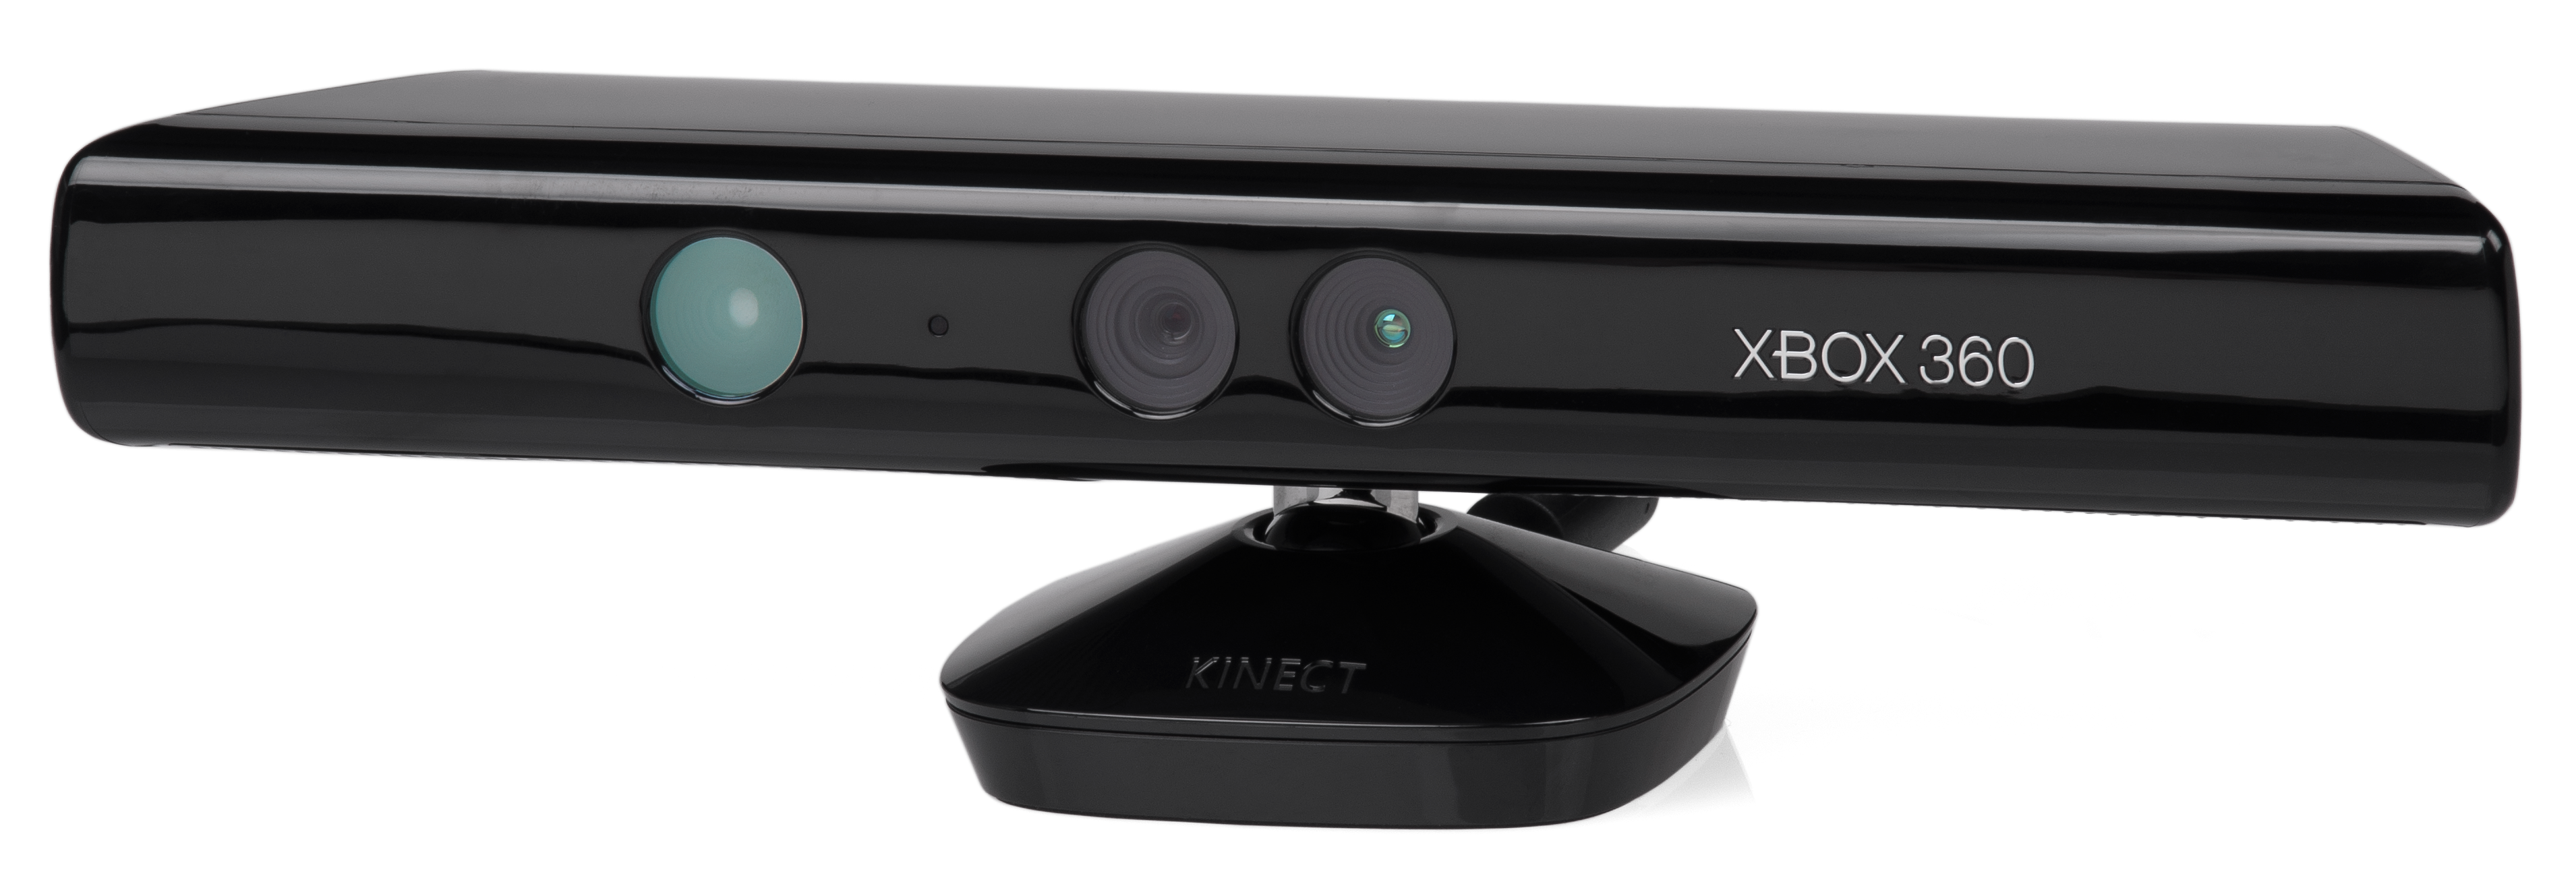
\includegraphics[width=0.4\textwidth]{kinect}
\caption{The Microsoft Kinect sensor is equipped with a depth camera that can "see" the positions and motion of human limbs.}
\label{fig:kinect}
\end{figure}

There are a variety of computing applications where the non-intrusive detection of human limb positions can be desirable as an input modality. Gaming is an obvious one (see Figure~\ref{fig:kinect-gaming}), where using movements with "prior mappings" to real-world happenings increases immersion \parencite{Cairns:2014}. Another one is user interfaces on public interactive systems: An input modality that does not require physical contact is often cheaper to deploy and maintain, and more hygienic to use. Of course, there are numerous other contexts where hygene considerations make a touchless interface may be desirable: Cooking, gardening, working on a dirty mechanism, and performing surgery \parencite{Wen:2013} come to mind. Other applications for perceptual interfaces include convenient control of smart homes \parencite{Tang:2013}, interactive art and musical instruments\footnote{\href{http://vimeo.com/45417241}{vimeo.com/45417241}}, interfaces for manipulating 3D images \parencite{Gallo:2013}, and spatial medicine \parencite{Lozano-Quilis:2013, Huang:2011, Simmons:2013}.

\begin{figure}[ht]
\centering
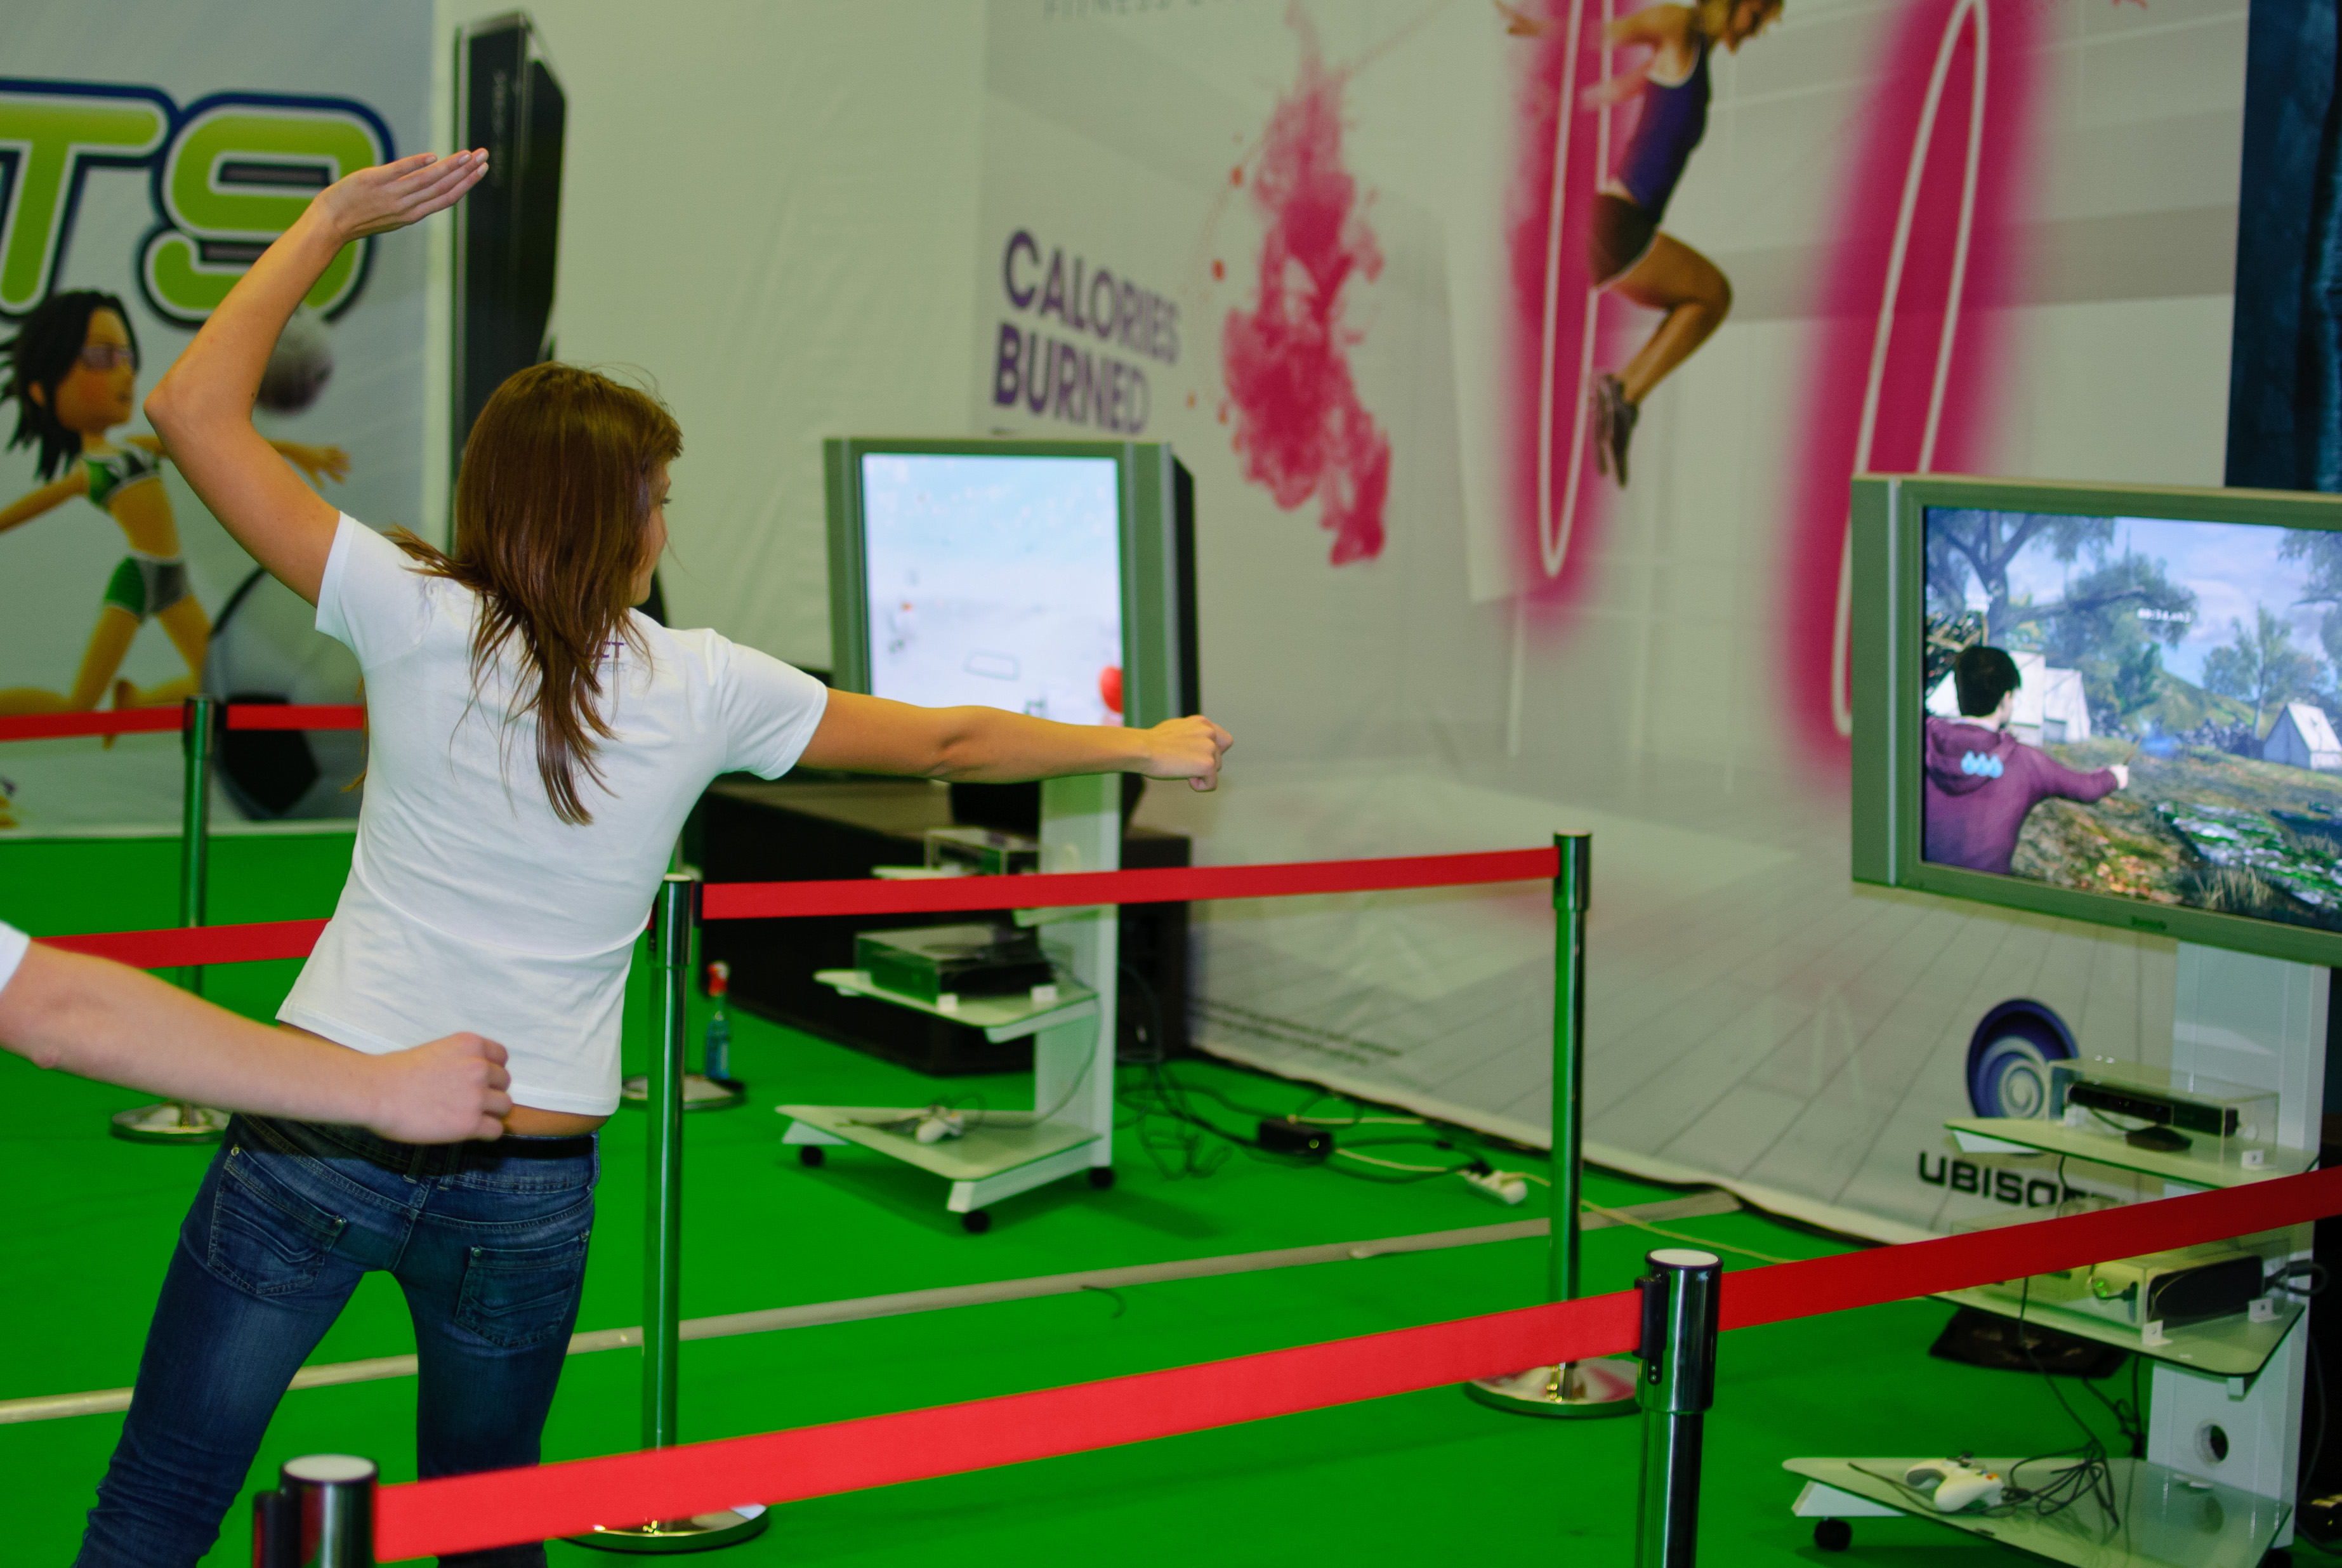
\includegraphics[width=0.8\textwidth]{kinect-gaming}
\caption{Gaming with the Microsoft Kinect.}
\label{fig:kinect-gaming}
\end{figure}

The design and development of perceptual interfaces requires that \emph{gestures} - limb positions and movements that constitute inputs to the interface - be \emph{authored} in a machine-readable manner and mapped to events within the interactive system. This can be done in a textual programming environment using tools supplied by vendors of gesture-sensing hardware\footnote{\href{http://www.microsoft.com/en-us/kinectforwindowsdev/}{microsoft.com/en-us/kinectforwindowsdev}}\footnote{\href{http://www.softkinetic.com}{softkinetic.com}} or third parties\footnote{\href{http://kinecttoolbox.codeplex.com}{kinecttoolbox.codeplex.com}}. Using textual programming to author gestures, however, has drawbacks - both for adept software developers and for comparatively non-technical users such as designers, artists, hobbyists or researchers in fields other than computing. (I will henceforth refer to these users who produce software not as an end, but as a means towards goals in their own domain, as \emph{end-users} \parencite{Ko:2011}). Specifically; for end-users, textual programming embodies a significant \emph{gulf of execution} – a chasm between the user's goals and the actions taken within a system to achieve those goals – since it introduces additional tasks like setting up the programming environment and getting used to the development ecosystem. For both end-users and software developers, textual programming embodies a significant \emph{gulf of evaluation} - a gap between a system's output and the users's expectations and intentions - since they do not fully support the embodied \parencite{Dourish:2004},  reflective \parencite{Schon:1984}, and experiential \parencite{Lindell:2014} practices inherent in the design, construction and evaluation \parencite{Hartmann:2006} of these highly interactive artifacts \parencite{Myers:2000, Lim:2008}. (See Figure~\ref{fig:gulfs} for a visualization of the \emph{gulf of execution} and the \emph{gulf of evaluation}. See \parencite{Norman:1986, Norman:2002} for a detailed discussion on the gulfs.)

\begin{figure}[ht]
\centering
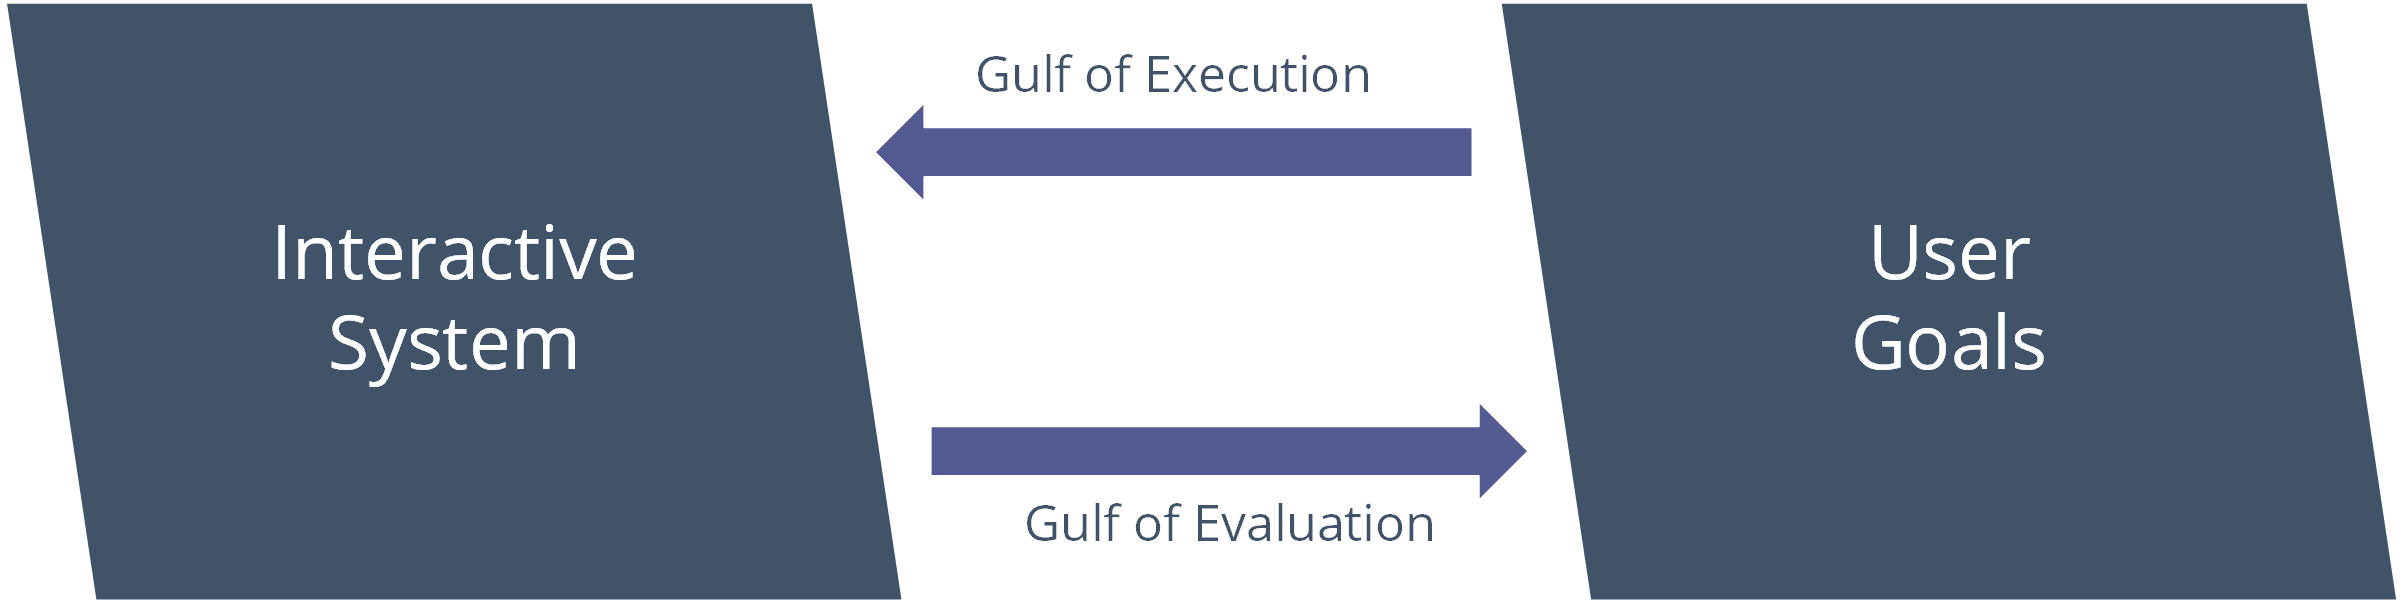
\includegraphics[width=0.8\textwidth]{gulfs}
\caption{The \emph{gulf of execution} and the \emph{gulf of evaluation}. The gulfs pertain to unidirectional aspects of interaction: The \emph{gulf of execution} lies between the user's goals and the interactive system; the \emph{gulf of evaluation} divorces the interactive system from the users's expectations and intentions.}
\label{fig:gulfs}
\end{figure}

Using appropriate tools for a job helps bridge the gulfs of evaluation and execution.

This thesis presents my attempt at producing an appropriate tool to support the design and development of perceptual gesture-based interfaces by end-users.

\section{Scope} %---------------------------------------------------------------

In human-computer interaction (HCI) and interaction design (IxD) literature, the usage of the word \emph{gesture} is ambiguous: Depending on the context, it may denote finger strokes on a touchscreen \parencite{Lu:2013}, deformations inflicted on a tangible input device \parencite{Warren:2013}, full-body poses \parencite{Walter:2013}, even finger movements on a keyboard \parencite{Zhang:2014}. For the purporses of this manuscript; the following definition, adapted from \cite{Kurtenbach:1990}, will be used:

\begin{quote}
\emph{A gesture is a movement or position of a human body part that conveys information.}
\end{quote}

By design, in order to accomodate existing works, this definition is broad. It allows for the use of any body part in gesturing as well as the use of sensing devices such as mouse, styli and gloves. It does not require an explicit intention to justify gesturing, thus accommodating non-command user interfaces \parencite{Nielsen:1993} such as those that respond to affective \parencite{Kapur:2005} and habitual \parencite{Liu:2009} gestures.

More specifically, I use the term \emph{mid-air gesture} to denote gestures that carry the following two characteristics:

\begin{enumerate}
\item The gesture should be performed in a volume where limbs can move freely in 3 dimensions; e.g. free space. This excludes gestures that are constrained to affect a tangible medium; e.g. a keyboard, a touch-sensitive surface, or a shape display \parencite{Follmer:2013}.
\item The gesture-sensing hardware should detect the movements and/or location of human body parts perceptually, without requiring physical contact; e.g. with a camera. This excludes systems that sense gestures using devices that must be worn, wielded, or touched; e.g. a mouse, a ring\footnote{\href{http://www.wearfin.com/}{wearfin.com}}\footnote{\href{https://www.hellonod.com/}{hellonod.com}}\footnote{\href{http://logbar.jp/ring/}{logbar.jp/ring}}, or an accelerometer \parencite{Kela:2006, Ashbrook:2010}.
\end{enumerate}

The gesture sensing input device used during the course of this work was a Microsoft \emph{Kinect for Xbox 360}; chosen due to its availability. The device employs an infrared projector-camera pair to capture 3D \emph{depth images}. If what resembles a typical human body is present in the depth image, the positions (relative to the sensor) of its large limbs are detected using machine learning \parencite{Girshick:2011, Shotton:2011, Shotton:2012, Shotton:2013}. A \emph{skeletal model} of the user is produced in this fashion (Figure~\ref{fig:intro-skeleton}). The alignment and motion of the skeletal model is then used to to control interactive applications.

\begin{figure}[ht]
\centering
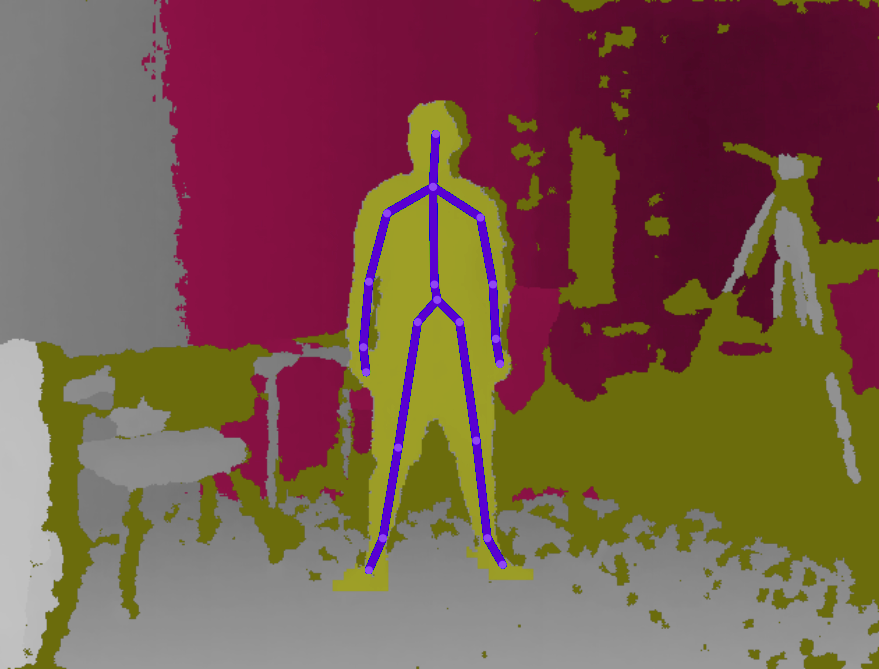
\includegraphics[width=0.8\textwidth]{intro-skeleton}
\caption{Skeletal tracking from a depth image.}
\label{fig:intro-skeleton}
\end{figure}

The Microsoft \emph{Kinect for Windows Software Development Kit (SDK)} version 1.8 was used to implement gesture sensing. The capabilities of the Kinect sensor and the SDK are not limited to skeletal tracking; they also include the detection of hand gestures, speech recognition, background removal from videos, facilitating proxemic interaction \parencite{Ballendat:2010}, fusing color and 3D images, and fusing data from multiple sensors\footnote{\href{http://blogs.msdn.com/b/kinectforwindows/archive/2013/09/17/updated-sdk-with-html5-kinect-fusion-improvements-and-more.aspx}{blogs.msdn.com/b/kinectforwindows/archive/2013/09/17/updated-sdk-with-html5-kinect-fusion-improvements-and-more.aspx}}. These topics, however, lie outside the scope of this work.

In kinesiology, human movements are classified according to movement precision \parencite{Haibach:2011}: \emph{Gross motor skills} denote large and comparatively imprecise movements produced by large muscles; e.g. jumping, or lifting weights. \emph{Fine motor skills} involve smaller movements with higher accuracy and precision; e.g. typing, or writing. Note that gestures do not always belong strictly to one of two discrete classes. Rather, the distinction between fine and gross gestures forms a continuum characterized by the size of the engaged musculature and the trade-off between force and precision \parencite{Edwards:2010} (Figure~\ref{fig:fine-gross-continuum}). One limitation of the skeletal tracking technology used for this work is that it can only detect gross gestures\footnote{Currently, the Kinect SDK does have support for hand gestures. However, this feature was not available while the design work described in this thesis was done.}. Thus, this work deals only with issues related to the use of \emph{gross movements} of the human limbs as an interaction modality in computing.

\begin{figure}[ht]
\centering
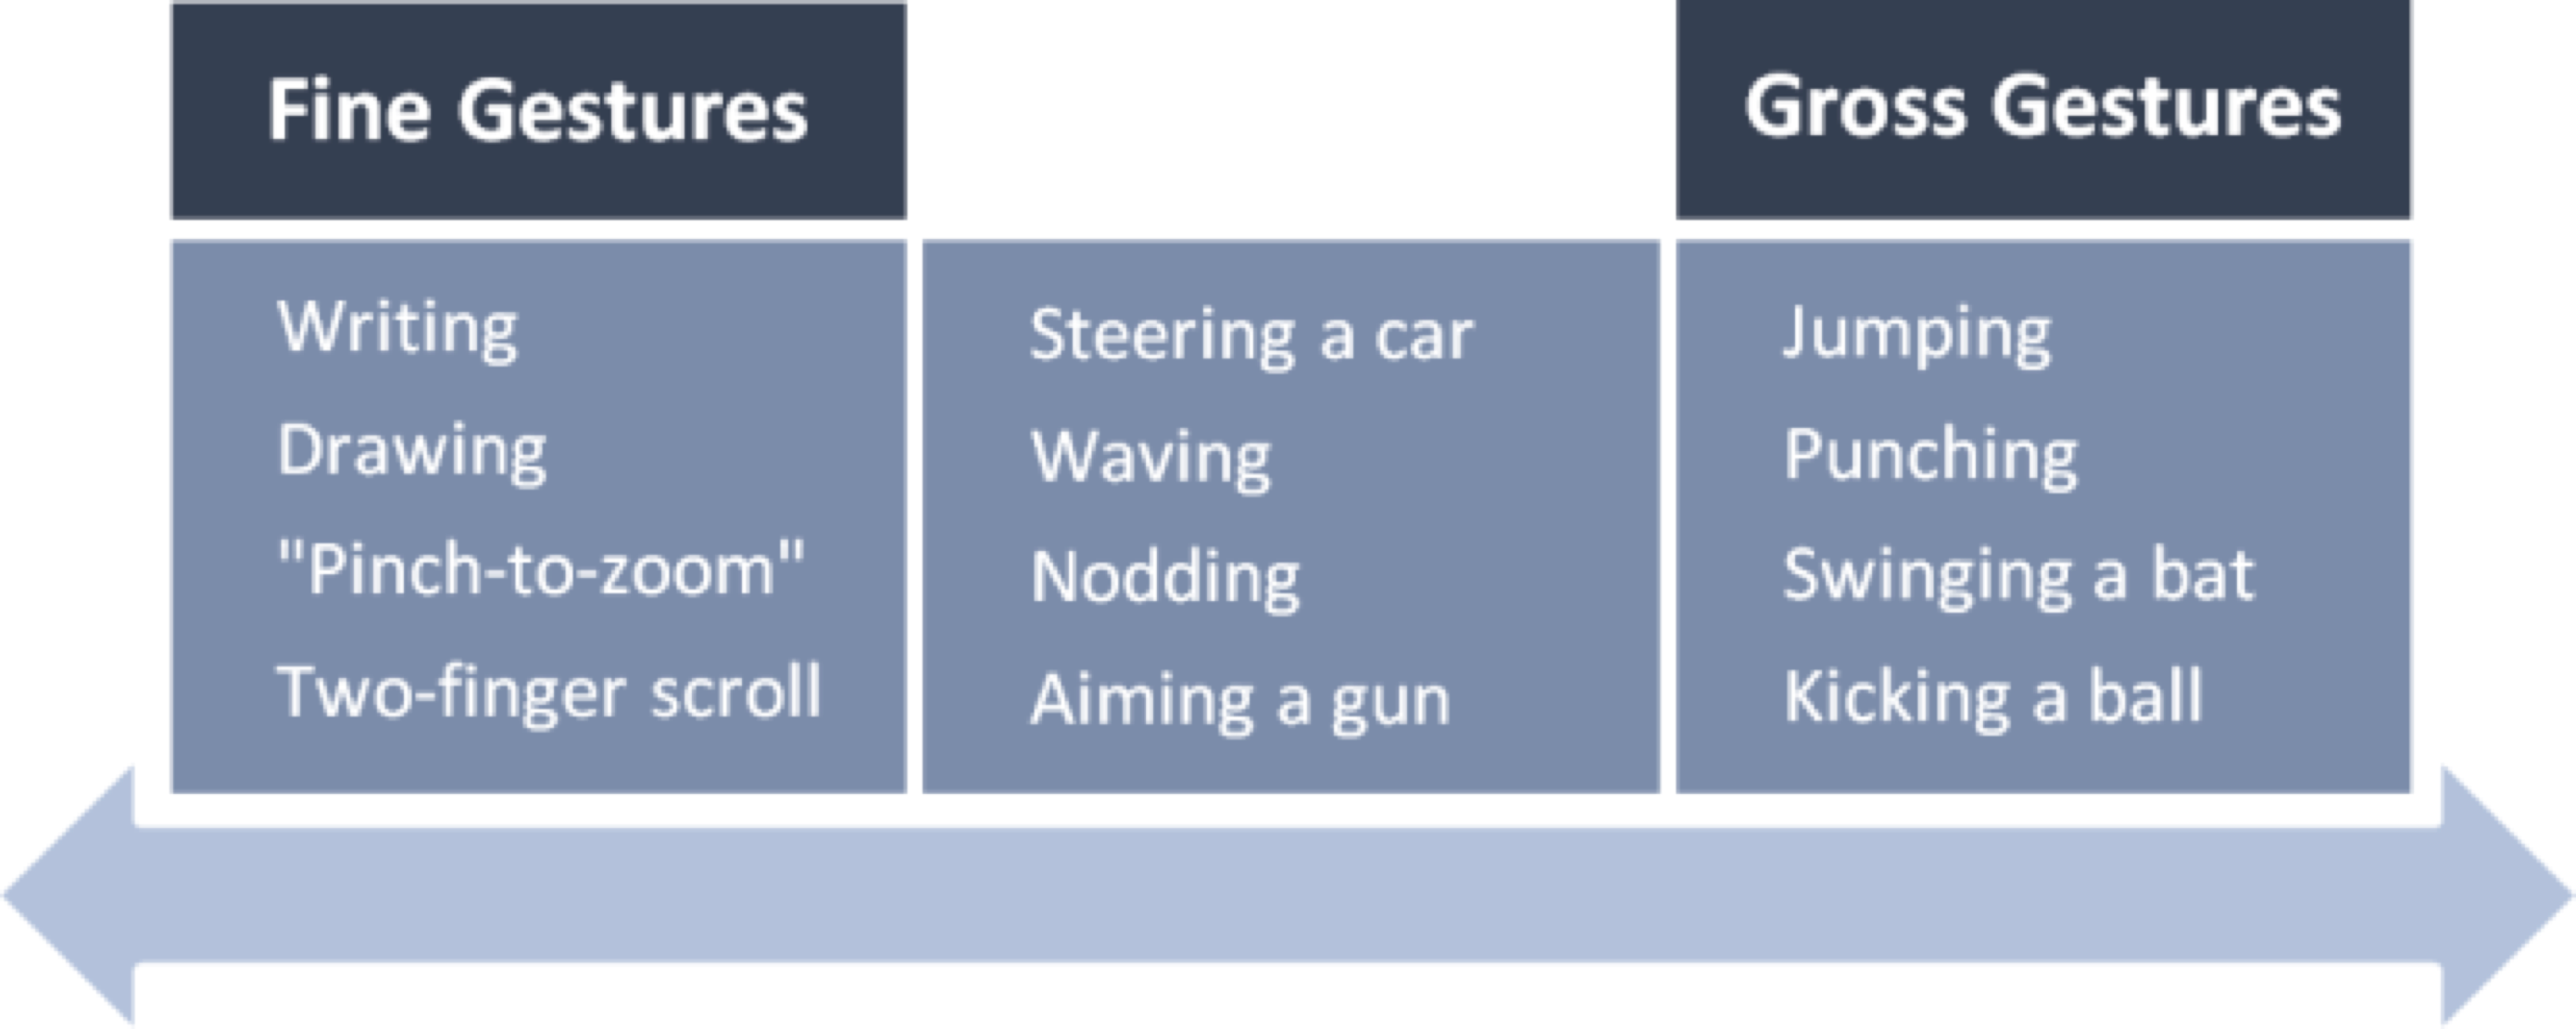
\includegraphics[width=0.8\textwidth]{fine-gross-continuum}
\caption{The continuum of \emph{fine} vs. \emph{gross} movements.}
\label{fig:fine-gross-continuum}
\end{figure}

In sum, the scope of this work covers the design and development of a \emph{software tool for authoring gross mid-air gestures} for interactive computing systems that employ \emph{skeleton tracking perceptual input devices}.

\section{Aim} %-----------------------------------------------------------------

The aim of this thesis is to document the design, development, deployment and evaluation of a \emph{software application for authoring gross mid-air gestures} for \emph{skeletal tracking perceptual input devices}.

The features and the user interface of this application are geared towards supporting the activities of \emph{end-users} rather than adept computer programmers. The methods employed in the design and evaluation of the application are selected to be appropriate for this purpose. The practices employed for the construction and deployment of the application also reflect its end-user focus: The application must perform well and reliably on users' computers, be easy to obtain and set up, and be maintainable to facilitate rapid adaptation to evolving technologies and user needs \parencite{McConnell:2009, Brooks:1995}.

\subsection{Research Questions} %-----------------------------------------------

The main research question pursued in this thesis is as follows:

\begin{center}
\emph{How can end-users' authoring of gross mid-air gestures for skeletal tracking interfaces be supported with a software tool?}
\end{center}

The main question breaks down into the following sub-questions that align with the research activities:

\begin{itemize}
\item What are the desiderata and design considerations that would pertain to mid-air gesture authoring software for end-users?
\item What methods should be used to elicit the desiderata and design considerations from the target users?
\item What are the technical considerations that would pertain to the application?
\item What methods are appropriate to evaluate the application?
\end{itemize}

\subsection{Hypothesis and Expected Result} %----------------------------------

I hypothesize that a suitably designed gesture authoring tool will accomplish the following:

\begin{itemize}
\item It will enable \emph{end-users} with no experience in textual programming and/or gestural interfaces to introduce gesture control to computing applications that serve their own goals.
\item It will provide \emph{developers} and \emph{designers} of gestural interfaces with a rapid prototyping tool that can be used to experientially evaluate designs.
\item By providing an appropriate representation of the design space, it will expose the capabilities and limitations of the technology and be fit to serve \emph{educational} purposes.
\end{itemize}

This application constitutes an artifact of \emph{research through design} \parencite{Frayling:1993}. Thus it is expected to fullfill the following criteria proposed in \cite{Zimmerman:2007}:

\begin{itemize}
\item \emph{Process.} The methods employed must be selected rationally and documented rigorously.
\item \emph{Invention.} Various topics must be integrated in a novel fashion to create the artifact.
\item \emph{Relevance.} The artifact must be situated within a real, current context; while supporting a shift towards a justifiably preferable state.
\item \emph{Extensibility.} The work must enable the future exploitation of the knowledge derived from it.
\end{itemize}

The expected result from this work is a software application that will accomplish the goals above and constitue an authentic contribution as an artifact of research through design.


\chapter{Background and Related Work}
\section{Gestural Interaction}

\subsection{Gesture Recognition}

\subsection{Gestural Interaction Design}

\section{End-User Programming}
\label{sec:end-user-programming}

"Programming" can be defined as "the process of transforming a mental plan of desired actions for a computer into a representation that can be understood by the computer" \parencite{Myers:2006}. The study of various aspects of programming has been a long-established topic of human-computer interaction research. Traditionally, the focus of this field has been on the activities of professional programmers and novices who are aiming to become professionals. A relatively recent topic of interest is the study of end-user programming as a topic distinct from the activities of professional and novice software developers \parencite{Myers:2006}. As such, interaction with a diverse array of devices --- e.g. TVs, telephones, alarm clocks... --- and a diverse assortment of tasks comprise topics of interest for programming research.

What differentiates an end-user from a professional programmer is their \emph{goals}: Professionals create and maintain software as an end, while end-users produce and customize software artifacts to support their own goals in some other domain \parencite{Ko:2011}. In many domains, the case for end-user programming --- rather than entrusting all development to professionals --- is mainly economical:  \textcite{Wulf:2004} argue that support for end-user programming makes software investments more efficient since empowering end-users to customize software mitigates the need for expensive development teams and processes (see Figure~\ref{fig:eud}). The effect is significant, since end-users outnumber professional programmers by orders of magnitude \parencite{Scaffidi:2005}. From a user-focused perspective, research on end-user programming is motivated by usability and engagement concerns \parencite{Germonprez:2007}; as well as the simple fact that some systems such as smart homes \parencite{Blackwell:2004} and health-related applications \parencite{Rizzo:2011, Lange:2011} must be customizable to suit individual needs \parencite{Holloway:2010}.

\begin{SCfigure}[\sidecaptionrelwidth][ht]
\centering
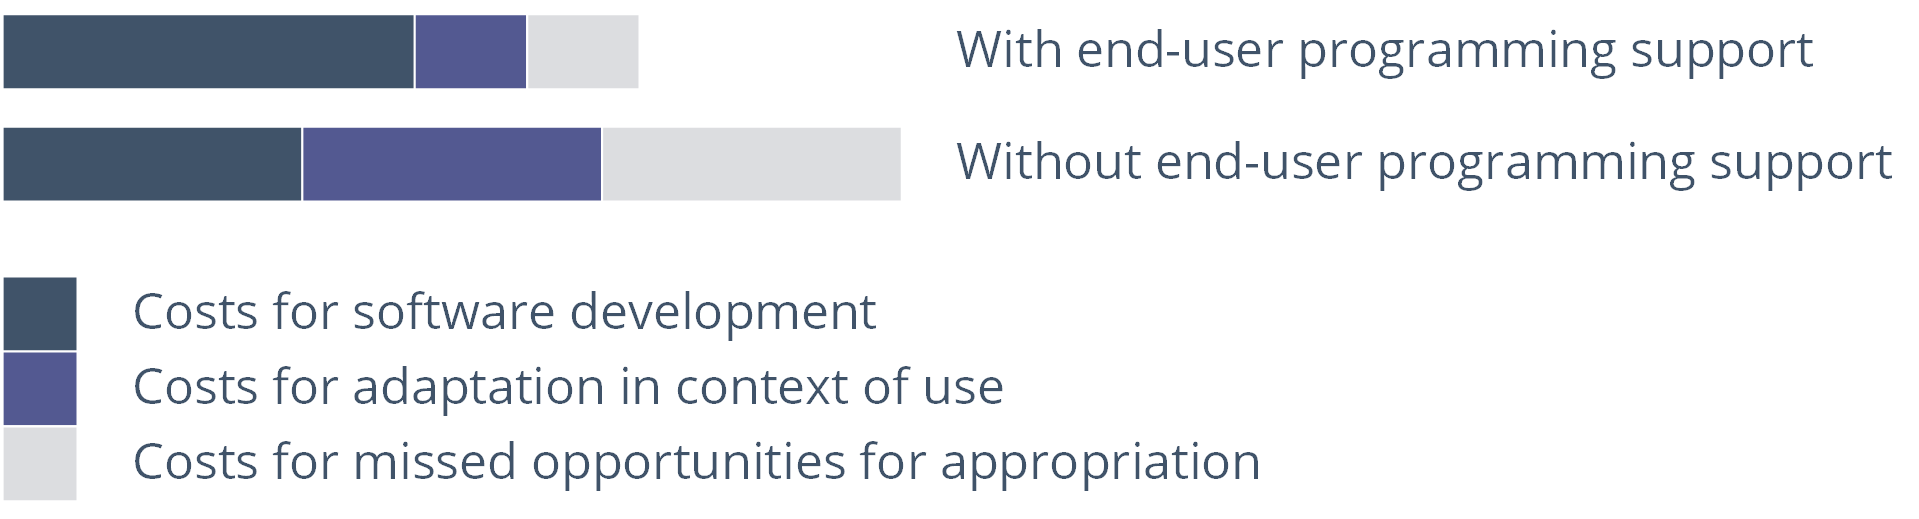
\includegraphics[width=0.7\textwidth]{eud}
\caption{Comparing the cost structure for software development, adaptation and appropriation with and without end-user programming support. Adapted from \textcite{Wulf:2004}.}
\label{fig:eud}
\end{SCfigure}

This thesis covers the design and development of a gesture authoring tool for designers' prototyping novel user interfaces and end-users' extending existing interfaces with the ability to recognize and respond to custom mid-air gestures. Various works on end-user programming that inform this effort are discussed below. A complete survey of this field is beyond the scope of this work; I recommend surveys by \textcite{Paterno:2013}; and \textcite{Myers:2006} as a starting point for the interested reader.

\subsection{Visual Programming}

\subsection{Programming by Demonstation}

\subsection{Programming Environments}

\subsection{End-User Software Engineering}

One strand of research on end-user programming considers issues beyond the construction and customization of software; e.g. design, testing, debugging, integration, reuse, and security. This strand, called \emph{end-user software engineering}, aims improve the \emph{quality} of software artifacts produced by end-users by leveraging knowledge derived from professional software engineering. A comprehensive review of this research is beyond the scope of this thesis. While end-users' design, specification, testing, debugging, and reuse of software artifacts are indeed relevant for a gesture authoring tool; this thesis  (as Chapter~\ref{chp:method} describes) approaches such issues from a design --- rather than software engineering --- perspective. For the reader interested in end-user software engineering, I recommend surveys by \textcite{Burnett:2004}, and \textcite{Ko:2011}.

\subsection{Psychological Issues}

A number of end-user programming researchers focus on psychological and cognitive issues that relate to end-user programmers. One objective for such research, as \textcite{Blackwell:2006} declares in his survey of the field, is "to increase our understanding of human cognition by studying a rather extreme domain of reasoning." Another objective is to tackle quality issues by informing the design of end-user programming tools and methods. Topics of interest include the difficulties of learning \parencite{Ko:2004, Pea:1987} and performing \parencite{Lewis:1987} programming-related tasks, and how people envision programming concepts \parencite{Pane:2001}.

\subsubsection{Learning Barriers}

From among research on the psychology of programming, particularly relevant for a gesture authoring tool is work by \textcite{Ko:2004} where the authors identify six "learning barriers" that obstruct end-user programmers across a variety of contexts:

\begin{enumerate}
\item \emph{Design barriers} are difficulties that are inherent in a problem, independent from how the solution is represented. They represent the inability of a learner to construct a solution to a given problem, which must be accomplished before the solution is implemented as software.
\item \emph{Selection barriers} impede learners from discovering what components are afforded by the programming environment, and which of those can be used to implement their design for a software solution.
\item \emph{Coordination barriers} hinder learners' understanding of how various components offered by the programming environment can be combined to achieve desired behaviors.
\item \emph{Use barriers} obscure the intent, usage and effects of programming components. To illustrate with an example: a learner may have determined that they need to use a "list" structure to implement an algorithm, but they may not know how to declare and initialize one within the programming environment.
\item \emph{Understanding barriers} arise when learners are not able to compare the external behavior, i.e. the results, of the software with their expectations. This is usually a result of an absence or inadequacy of feedback as to what the software does or does not do.
\item \emph{Information barriers} disrupt learners' understanding of the internal workings of the software. They manifest as learners' inability to test hypotheses they might have about how the software does what it does.
\end{enumerate}

The authors relate these learning barriers to \posscite{Norman:1986, Norman:2002} concepts of the \emph{gulf of execution} and the \emph{gulf of evaluation} (which I described in section~\ref{sec:motivation} to motivate the development of a gesture authoring tool). Specifically, they explicate that \emph{design}, \emph{coordination}, and \emph{use} barriers spawn gulfs of \emph{execution}; \emph{understanding} barriers pose gulfs of \emph{evaluation}; while \emph{selection} and \emph{information} barriers constitute gulfs of \emph{execution} and \emph{evaluation}. The authors recommend adapting \posscite{Norman:2002} recommendations for bridging the gulfs and overcoming the learning barriers.

\subsubsection{Attention Investment}

\section{Authoring Mid-Air Gestures}

This section presents an overview of prior research on gesture authoring tools which has influenced my design. While development tools provided by vendors of gesture-sensing hardware focus on supporting textual programming, ongoing research suggests a set of diverse approaches to the problem of how to represent and manipulate three-dimensional gesture data. Existing works approach the issue in three ways that constitute distinct paradigms for visually authoring mid-air gestures. These are:

\begin{enumerate}
\item Using 2-dimensional graphs of the data from the sensors that detect movement;
\item using a visual markup language; and,
\item representing movement information using a timeline of
frames.
\end{enumerate}

In addition, there are approaches to manipulating gesture information that rely predominantly on textual representations.

These paradigms for visualizing and manipulating gesture data often interact with two approaches to authoring gesture information:

\begin{itemize}
\item Authoring gestures by \emph{declaration} involves the use of a high-level syntax to describe gesture information without specifying a computational control flow.
\item Authoring gestures by \emph{demonstration} is done by recording one or more examples and employing machine learning techniques to train a recognizer.
\end{itemize}

In addition, gestures can be defined through \emph{imperative} programming, in terms of a sequence of states or actions. This is the standard approach for authoring gestures in general-purpose textual programming environments. From a design perspective, this approach embodies significant gulfs of execution and evaluation, while erecting learning barriers for end-users (see Sections~\ref{sec:motivation}~and~\ref{sec:end-user-programming}). Imperative authoring of gestures is also suboptimal from a software engineering perspective (see Section~\ref{sec:motivation}; as well as \textcite{Hoste:2014}). Thus, imperative textual programming has not influenced my design significantly.

The three visual authoring paradigms enumerated above do not have to be used exclusively, and nor do demonstration and declarative programming. Aspects of different paradigms may find their place within the same user interface. A popular approach, for example, is to introduce gestures by demonstration, convert gesture data into a visual representation, and then declaratively modify it.

Below, I use examples from the literature to elaborate on the approaches enumerated above. I comment on their strengths and weaknesses based on previously published evaluations conducted with software that implement them.

Some of the work discussed below pertains to gesture-sensing systems which employ intrusive methods (e.g. markers or inertial sensors) rather than perceptual input devices. Even though the scope of this thesis does not fully encompass the intrusive sensing of mid-air gestures; the user interfaces of gesture authoring applications for intrusive sensors have aspects that inform the design of an authoring tool for perceptual interfaces. Thus, tools that target intrusive sensing applications and tools for perceptual interfaces are both considered.

\subsection{Using Graphs of Movement Data}

Visualizing and manipulating movement data using 2-dimensional graphs that represent low-level kinematic information is a popular approach for authoring mid-air gestures. This approach is often preferred when gesture detection is performed using inertial sensors such as accelerometers and gyroscopes. It also accommodates other sensors that read continuously variable data such as bending, light and pressure. Commonly the horizontal axis of the graph represents time while the vertical axis corresponds to the reading from the sensor. Often a “multi-waveform” occupies the graph, in order to represent data coming in from multiple axes of the sensor. Below, we study three software tools that implement graphs for representing gesture data: \emph{Exemplar}, \emph{MAGIC} and \emph{GIDE}.

\subsubsection{Exemplar}

\emph{Exemplar} \parencite{Hartmann:2007} relies on \emph{demonstration} to acquire gesture data and from a variety of sensors - accelerometers, switches, light sensors, bend sensors, pressure sensors and joysticks. Once a signal is acquired via demonstration, on the resulting graph, the developer marks the area of interest that corresponds to the desired gesture. The developer may interactively apply filters on the signal for offset, scaling, smoothing and first-order differentiation. \emph{Exemplar} offers two methods for recognition: One is pattern matching, where the developer introduces many examples of a gesture using the aforementioned method and new input is compared to the examples. The other is thresholding, where the developer manually introduces thresholds on the raw or filtered graph and gestures are recognized when motion data falls between the thresholds. This type of thresholding also supports hysteresis, where the developer introduces multiple thresholds that must be crossed for a gesture to be registered.

\emph{Exemplar}’s user studies suggest that this implementation of the paradigm is successful in increasing developer engagement with the workings and limitations of the sensors used. Possible areas of improvement include a technique to visualize multiple sensor visualizations and events and finer control over timing for pattern matching.

\subsubsection{MAGIC}

\posscite{Ashbrook:2010} \emph{System for Multiple Action Gesture Interface Creation (MAGIC)} is another tool that implements the 2-dimensional graphing paradigm. The focus of \emph{MAGIC} is programming by \emph{demonstration}. It supports the creation of training sets with multiple examples of the same gesture. It allows the developer to that keep track of the internal consistency of the provided training set; and check against conflicts with other gestures in the vocabulary and an “Everyday Gesture Library” of unintentional, automatic gestures that users perform during daily activities. \emph{MAGIC} uses the graph paradigm only to visualize gesture data and does not support manipulation on the graph.

One important feature in \emph{MAGIC} is that the motion data graph may be augmented by a video of the gesture example being performed. Results from user studies indicate that this feature has been highly favored by users, during both gesture recording and retrospection. Interestingly, it is reported that the “least-used visualization [in \emph{MAGIC}] was the recorded accelerometer graph;” with most users being “unable to connect the shape of the three lines [that correspond to the 3 axes of the accelerometer reading] to the arm and wrist movements that produced them.” Features preferred by developers turned out to be the videos, “goodness” scores assigned to each gesture according to how they match gestures in and not in their own class, and a sorted list depicting the “distance” of a selected example to every other example.

\subsubsection{GIDE}

\emph{Gesture Interaction Designer (GIDE)} by \textcite{Zamborlin:2014} features an implementation of the graph paradigm for authoring accelerometer-based mid-air gestures. \emph{GIDE} leverages a “modified” hidden Markov model approach to learn from a single example for each gesture in the vocabulary. The user interface implements two distinct features: (1) Each gesture in the vocabulary is housed in a “gesture editor” component which contains the sensor waveform, a video of the gesture being performed, an audio waveform recorded during the performance, and other information related to the gesture. (2) A “follow” mode allows the developer to perform gestures and get real- time feedback on the system’s estimate of which gesture is being performed (via transparency and color) and where they are within that gesture. This feedback on the temporal position within a gesture is multimodal: The sensor multi-waveform, the video and the audio waveform from the video are aligned and follow the gestural input. \emph{GIDE} also supports “batch testing” by recording a continuous performance of multiple gestures and running it against the whole vocabulary to check if the correct gestures are recognized at the correct times.

User studies on \emph{GIDE} reveal that the combination of multi- waveform, video and audio was useful in making sense of gesture data. Video was favored particularly since it allows developers to still remember the gestures they recorded after an extended period of not working on the gesture vocabulary. Another finding from the user studies was the suggestion that the “batch testing” feature where the developer records a continuous flow of many gestures to test against could be leveraged as a design strategy --- gestures could be extracted from a recorded performance of continuous movement.

\subsubsection{Discussion}

Graphs that display acceleration data seem to be the standard paradigm for representing mid-air gestures tracked using acceleration sensors. This paradigm supports direct manipulation for segmenting and filtering gesture data, but manipulating acceleration data directly to modify gestures is unwieldy. User studies show that graphs depicting accelerometer (multi-)waveforms are not effective as the sole representation of gesture information, but work well as a component within a multimodal representation along with video.

\subsection{Visual Markup Languages}

Using a visual markup language for authoring gestures can allow for rich expression and may accommodate a wide variety of gesture-tracking devices, e.g. accelerometers and skeletal tracking, at the same time. The syntax of these visual markup languages can be of varying degrees of complexity, but depending on the sensor(s) used for gesture detection, making use of the capabilities of the hardware may not require a very detailed syntax. Below, I examine a software tool, \emph{EventHurdle}, that implements a visual markup language for gesture authoring; and I discuss a gesture spotting approach based on control points which does not feature a concrete implementation, but provides valuable insight.

\subsubsection{EventHurdle}

\textcite{Kim:2013} describe a declarative hurdle-driven visual gesture markup language implemented in the \emph{EventHurdle} authoring tool. The \emph{EventHurdle} syntax supports gesture input from single-camera-based, physical sensor-based and touch-based gesture input. In lieu of a timeline or graph, \emph{EventHurdle} projects gesture trajectory onto a 2-dimensional workspace. The developer may perform the gestures, visualize the resulting trajectory on the workspace, and declaratively author gestures on the workspace by placing “hurdles” that intersect the gesture trajectory. Hurdles may be placed in ways that result in serial, parallel and/or recursive compositions. “False hurdles” are available for specifying unwanted trajectories. While an intuitive way to visualize movement data from pointing devices, touch gestures and blob detection; this approach does not support the full range of expression inherent in 3-dimensional mid-air gesturing.

Gestures defined in \emph{EventHurdle} are configurable to be location-sensitive or location-invariant. By design, orientation- and scale-invariance are not implemented in order to avoid unnecessary technical options that may distract from “design thinking.”

User studies on \emph{EventHurdle} comment that the concept of hurdles and paths is “easily understood” and it “supports advanced programming of gesture recognition.” Other than this, supporting features, rather than the strengths and weaknesses of the paradigm or comparison with other paradigms, have been the focus of user studies.

Worth noting is that \emph{EventHurdle} is implemented as a plug-in for Adobe Flash\footnote{\href{http://www.adobe.com/products/flash.html}{adobe.com/products/flash}}, which may pose as a barrier for users who have not invested in the software.

\subsubsection{Control Points}

\posscite{Hoste:2013} versatile and promising approach uses spatiotemporal constraints around control points to describe gesture trajectories. While the focus of the approach is on gesture spotting (i.e. the segmentation of a continuous trajectory into discrete gestures) and not gesture authoring, they do propose a human-readable and manipulable external representation. This external representation has significant expressive power and support for programming constructs such as negation (for declaring unwanted trajectories) and user-defined temporal constraints. While the authors’ approach is to infer control points for a desired gesture from an example, the representation they propose also enables the manual placement of control points.

The authors do not describe an authoring implementation that has been subjected to user studies. However, they discuss a number of concepts that add to the expressive power of using control points as a visual markup language to represent and manipulate gesture information. The first is that it is possible to add temporal constraints to the markup; i.e. a floor or ceiling value can be specified for the time taken by the tracked limb or device to travel between control points. This is demonstrated not on the graphical markup (which can be done easily), but on textual code generated to describe a gesture – another valuable feature. The second such concept is that the control points are surrounded by boundaries whose size can be adjusted to introduce spatial flexibility and accommodate “noisy” gestures. Third, boundaries can be set for negation when the variation in the gesture trajectory is too much. The authors discuss linear or planar negation boundaries only, but introducing negative control points into the syntax could also be explored. Finally, a “coupled recognition process” is introduced, where a trained classifier can be called to distinguish between potentially conflicting gestures; e.g. a circle and a rectangle that share the same control points.

One limitation of this approach is the lack of support for scale invariance. One way of introducing scale invariance may be to automatically scale boundary sizes and temporal constraints with the distance between control points. However, it is likely that the relationship between optimal values for these variables is nonlinear, which could make automatic scaling infeasible.

\subsubsection{Discussion}

The expressive power and usability of a visual markup language may vary drastically depending on the specifics of the language and the implementation. The general advantage of this paradigm is that it is suitable for describing and manipulating location-based gesture information (rather than acceleration-based information commonly depicted using graphs). This makes using a visual markup language suitable for mid-air gestures detected by depth-sensing cameras, where the interaction space is anchored to the sensor and the users' body parts move in relation to each other and the sensor. Either the motion sensing device or part of the skeletal model could be used to define a reference frame and gesture trajectories could be authored in a location-based manner using a visual markup language.

\subsection{Timelines}

Timelines of keyframes are commonly used in video editing applications. They often consist of a series of ordered thumbnails and/or markers that represent the content of the moving picture and any editing done on it, such as adding transitions. A collection of commercial\footnote{\href{http://www.gesturepak.com}{gesturepak.com}}$^{,}$\footnote{\href{http://www.gesturestudio.ca}{gesturestudio.ca}} and research \parencite{Tang:2013} efforts implement timelines along with demonstration for authoring skeletal tracking gestures. Introducing gestures via demonstration requires the temporal segmentation of intended gestures from intermediate movements to be done manually - this is accomplished through manual editing on a timeline of keyframes.

\subsubsection{Gesture Studio}

One application that implements a timeline to visualize gesture information is the commercial \emph{Gesture Studio}\footnote{\href{http://www.gesturestudio.ca}{gesturestudio.ca}}. The application works only with sensors that detect gestures through skeletal tracking using an infrared depth camera. Users introduce gestures in \emph{Gesture Studio} by demonstration, through performing and recording examples. The timeline is used to display thumbnails for each frame of the skeleton information coming from the depth sensor. The timeline is updated after the user finishes recording a gesture; while during recording, a rendering of the skeletal model tracked by the depth sensor provides feedback. After recording, the user may remove unwanted frames from the timeline to trim gesture data for segmentation. Reordering frames is not supported since gestures are captured at a high frame rate (depending on the sensor, usually around 30 frames per second), which would make manual frame-by-frame editing inconvenient. The process through which these features have been selected is opaque, since there are no published studies that present the design process or evaluate \emph{Gesture Studio} in use.

\subsubsection{Discussion}

In gesture authoring interfaces, timelines make sense when gesture tracking encompasses many limbs and dynamic movements that span more than a few seconds. Spatial and temporal concerns for gestures in two dimensions, such as those performed on surfaces, can be represented on the same workspace. The representation of mid-air gestures requires an additional component such as a timeline to show the change over time.

Timelines of keyframes are used often in conjunction with programming by \emph{demonstration}, for the manual segmentation of gesture data from intermediate bodily movements. For end-users without familiarity with machine learning concepts, the task of composing good training samples is not trivial. Moreover, this method cannot be used if the depth sensing device is not available during development (e.g. due to malfunction or devices being shared between users).

\subsection{Textual Approaches}

\subsubsection{FAAST}

For declaratively authoring mid-air gestures for skeletal tracking, the \emph{Flexible Action and Articulated Skeleton Toolkit (FAAST)} \parencite{Suma:2013} provides atomic \emph{action primitives} that can be used to compose rules in plain English such as "right hand above right shoulder by at least 20 cm." (Figure~\ref{fig:faast}) These constraints specify the position of, the speed of, or the angle between limbs, as well as general body orientation. \emph{FAAST} controls other applications on the computer via mapping gestures to keyboard and mouse events. While describing gestures using atomic rules affords significant expressive power, this representation does not embody a visualization of the constraints embedded in the design space and thus may not serve to bridge the gulf of execution that obstructs end-users.

\begin{SCfigure}[\sidecaptionrelwidth][ht]
\centering
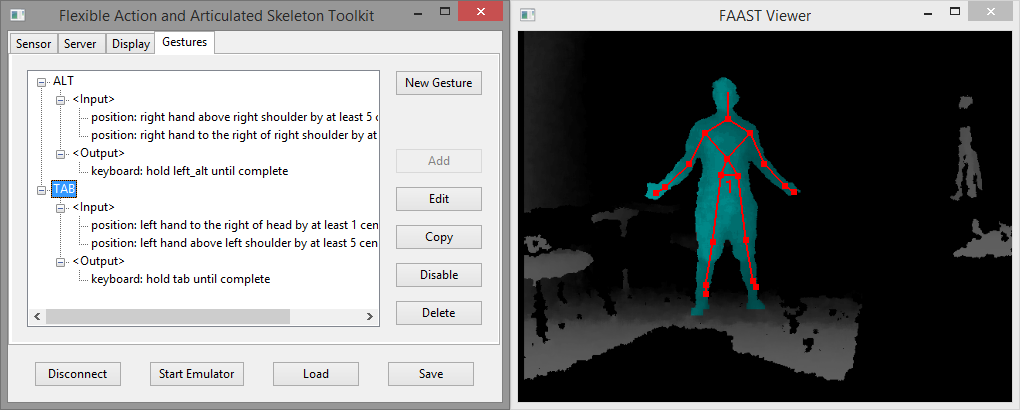
\includegraphics[width=0.8\textwidth]{faast}
\caption{FAAST \parencite{Suma:2013} provides atomic primitives that can be used to compose rules in plain English that map to mid-air gestures.}
\label{fig:faast}
\end{SCfigure}

\subsection{Discussion}

Above, tools that exemplify user interface paradigms for visually and textually authoring mid-air gestures have been presented (Table~\ref{tab:systems-summary}). For sensor-based gesturing, the standard paradigm used to represent gesture information appears to be projecting the sensor waveforms onto a graph. Graphs appear to work well as components that represent sensor- based gestures, allow experimentation with filters and gesture recognition methods, and support direct manipulation to some extent. User studies show that while the graphs alone may not allow developers to fully grasp the connection between movements and the waveform \parencite{Ashbrook:2010}, they have been deemed useful as part of a multimodal gesture representation \parencite{Zamborlin:2014}. Using hurdles as a visual markup language offers an intuitive and expressive medium for gesture authoring, but it is not able to depict fully 3-dimensional gestures. Using spherical control points may be more conducive to direct manipulation while still affording an expressive syntax, but no implementation of this paradigm exists for authoring mid-air gestures. Finally, timelines of frames may come in handy for visualizing dynamic gestures with many moving elements, such as in skeletal tracking; but used in this fashion they allow only visualization and not manipulation.

\begin{table}[ht]
\centering
\renewcommand{\arraystretch}{1.8}
\begin{tabular}{>{\raggedright\arraybackslash}m{.2\textwidth} >{\raggedright\arraybackslash}m{.2\textwidth} >{\raggedright\arraybackslash}m{.2\textwidth} >{\raggedright\arraybackslash}m{.28\textwidth}}
\textbf{System} &
\textbf{UI Paradigm} &
\textbf{Programming Approach} &
\textbf{Insights from Evaluation} \\
\hline
\textbf{Exemplar} \newline
\parencite{Hartmann:2007} &
Graphs &
Demonstration &
Increases engagement with sensor workings and limitations. \\
\textbf{MAGIC} \newline
\parencite{Ashbrook:2010} &
Graphs (multi-waveform) &
Demonstration &
Users unable to connect waveform to physical movements. Optional video is favored over graphs. \\
\textbf{GIDE} \newline
\parencite{Zamborlin:2014} &
Graphs (multi-waveform, with video) &
Demonstration &
Multimodal representation helps make sense of gesture data. \\
\textbf{EventHurdle} \newline
\parencite{Kim:2013} &
Visual markup language &
Declaration &
Easily understood. Supports “advanced” programming. \\
\textbf{Control Points} \newline
\parencite{Hoste:2013} &
Visual markup language &
Declaration and Demonstration &
Not implemented. \\
\textbf{Gesture Studio}\footnote{\href{http://www.gesturestudio.ca}{gesturestudio.ca}} &
Timeline &
Demonstration &
Not published. \\
\textbf{FAAST} \newline
\parencite{Suma:2013} &
Textual &
Declaration &
Widely adopted due to standalone, end-to-end implementation. \\
\hline
\end{tabular}
\caption{Summary of studies on systems that exemplify user interface paradigms for authoring mid-air gestures.}
\label{tab:systems-summary}
\end{table}


\chapter{Method}
\label{chp:method}
\section{Research Through Design}

\section{User-Centered Design}
\label{sec:user-centered-design}

\section{Design and Evaluation of User Interface Authoring Tools}

\textcite{Olsen:2007} argues that user interface design tools, particularly those that deal with unconventional interaction techniques (e.g. mid-air gesture sensing), do not lend themselves to conventional software evaluation methods. One reason for this is that such tools require domain-specific expertise, which --- by the nature of novel tools --- no user population possesses. Another reason is that these tools support complex tasks with high inter-user variability in terms of the users’ mental models of the tasks. “Meaningful comparisons between two tools for a realistically complex problem are confounded in so many ways as to make statistical comparisons more fantasy than fact.” \parencite{Olsen:2007} From the framework proposed by Olsen for the evaluation of user interface toolkits, I derived the following four guidelines to direct the design of my mid-air gesture authoring tool:

\begin{itemize}
\item \emph{Reduce development time.} A good authoring tool should allow for the rapid implementation of design changes. This can be encouraged by reducing the number of choices that have to be made to express a design. (Granted, there may exist a tradeoff between this concern and the expressive power of the authoring tool.)
\item \emph{Encapsulate and simplify expertise.} Considerable technical know-how is required to design and develop applications for emerging technologies. A good design tool liberates the designer from the need for prior knowledge, yet communicates the capabilities and limitations of the technology to nudge the designer towards feasible designs.
\item \emph{Lower skill barriers.} Empowering new populations of users to envision and implement designs “expands the set of people who can effectively create new applications.” \parencite{Olsen:2007}
\item \emph{Make use of a common infrastructure.} It is difficult to get users to adopt a new standard. As much as possible, authoring tools should hook up to existing and widely adopted tools and practices, and complement existing workflows; upgrading rather than negating the common denominator.
\end{itemize}

Employing a user interface paradigm for expressing design choices that reflects the problem being solved and embodies the constraints of the design space \parencite{Norman:1993} serves all four the guidelines above.

In addition, \textcite{Shoemaker:2010} propose design guidelines for body-centric interaction with large displays. From among the guidelines they propose, two generalize to influence the design of an authoring tool for mid-air gestures:

\begin{itemize}
\item Interaction using mid-air gestures at a distance should be \emph{“mediated through a representation that binds personal and extrapersonal space.”} A means for communicating the constraints and opportunities of the interaction space to the user is recommended for mid-air gestural interfaces. This holds for design tools that target these interactions.
\item It is recommended that \emph{users’ sense of proprioception be leveraged} by allowing some operations to be performed in the user’s personal space, without requiring visual feedback. In terms of authoring interactions, this guideline calls for encouraging gesture designs that capitalize on proprioception through the nature of the authoring paradigm.
\end{itemize}

In sum, six guidelines derived from previous work form the basis of my design rationale for the gesture authoring interface (Figure~\ref{fig:design-guidelines}). The first four, derived from \posscite{Olsen:2007} work, identify and address concerns that pertain to user interface design tools. The last two, derived from the work of \textcite{Shoemaker:2010}, attend to concerns related to perceptual interactions in general. Whether or not the final design for the authoring tool conforms to these guidelines is evaluated through user studies.

\begin{SCfigure}[\sidecaptionrelwidth][ht]
\centering
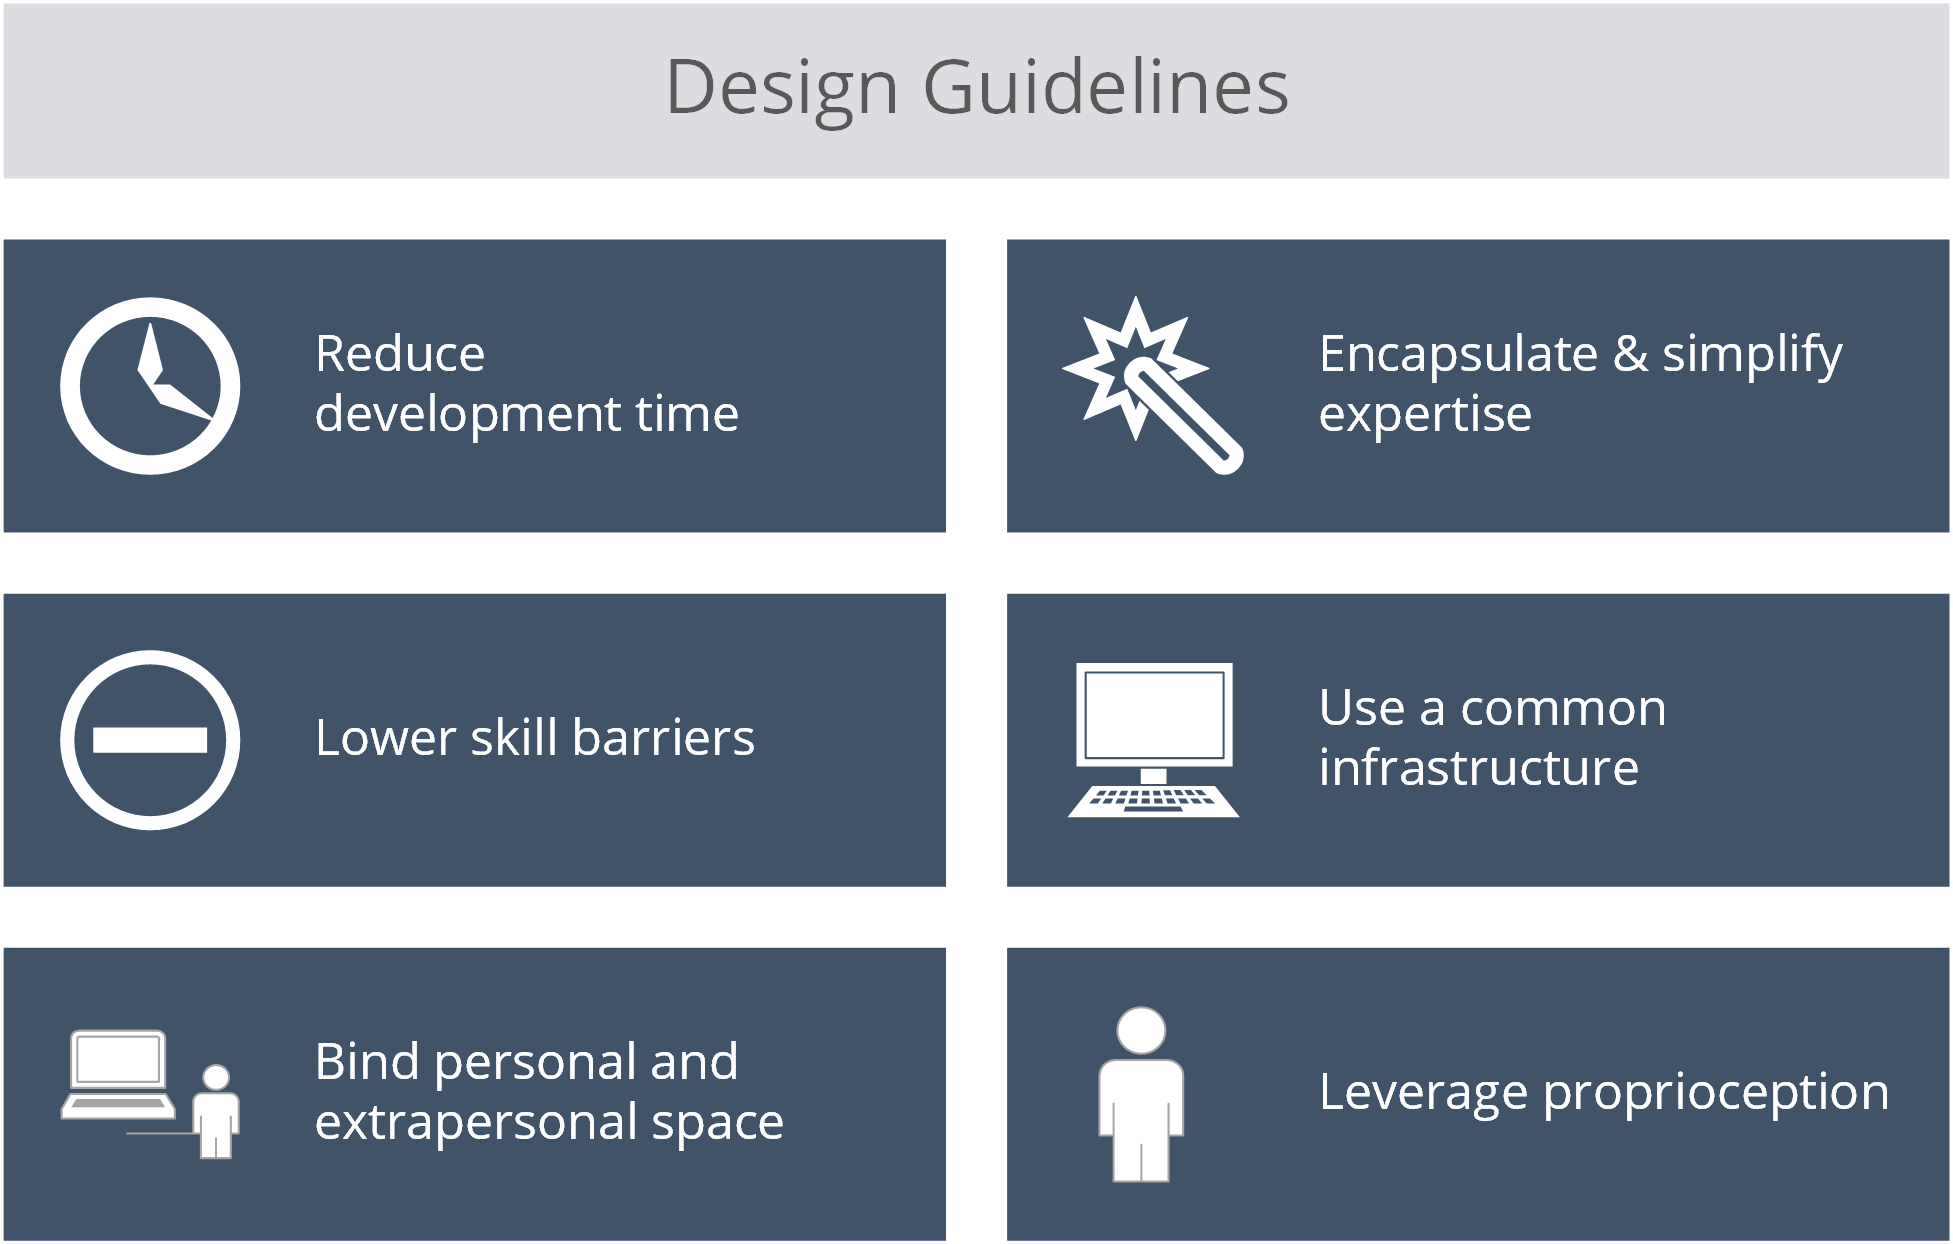
\includegraphics[width=0.7\textwidth]{design-guidelines}
\caption{Guidelines derived from the literature formed the basis of the design rationale for a gesture authoring tool.}
\label{fig:design-guidelines}
\end{SCfigure}

Additionally, from a programming perspective (see Section~\ref{sec:end-user-programming}); \textcite{Myers:2000} identify five themes that influence the success of user interface tools:

\begin{itemize}
\item User interface tools should strive to achieve a low \emph{threshold} --- i.e. be easy to learn --- and a high \emph{ceiling} --- i.e. significant expressive power.
\item Successful tools lead users to making the right choices and avoiding wrong designs by offering a well-designed \emph{path of least resistance}
\item A tool should embody \emph{predictability} and avoid unpredictable automatic operations.
\item Developers of user interface tools should stay on top of developments, since user interface technologies are \emph{moving targets} that can change significantly or become obsolete at a rapid pace.
\item A tool should only \emph{address the parts of the user interface that are needed}.
\end{itemize}

The first of these themes is specifically captured in part by Olsen's recommendations that a tool should lower skill barriers and empower new users. A high level of expressive power is desirable, but the weight of this concern will be governed by user needs (see Section~\ref{sec:user-centered-design}). The encapsulation and simplification of expertise, along with the use of user-centered design tools and methods, integrate all of these themes.


\chapter{Hotspotizer: Description}
This chapter describes a novel user interface paradigm for authoring mid-air gestures based on \emph{space discretization}, and its implementation as part of an end-to-end software tool designed to support end-users: \emph{Hotspotizer}. The design of the user interface paradigm

\section{Space Discretization}

Hotspotizer implements a paradigm based on space discretization for visualizing and manipulating gesture information. In the current implementation, we partition the space around the skeletal model tracked by the Kinect sensor into cubes that are 15cm on each side.

The total workspace is a large cube that is 3m on each side. While this is much larger than both the horizontal and vertical reach of many people; this is by design, to accommodates unusually tall users. The centroid of the cube that comprises the workspace is affixed to the "hip center" joint returned by the Kinect sensor. By specifying and tracking joint movements relative to the user’s skeletal model rather than the sensor’s position in real space, we aimed to leverage the user’s sense of proprioception \parencite{Shoemaker:2010} in gesturing.

To describe gestures, the cubic cells within the workspace may be marked to become hotspots – or \emph{hotspotized} – that register when a specified joint passes through them. Joints available for tracking are the hands, feet, elbows, knees and the head. Hotspotizing is accomplished by using front and side views in the Editor workspace. The front view is used to specify the horizontal and vertical positions of the hotspots. The side view is used to confirm the vertical and specify depth-wise positions. The design of this interaction style was inspired by architectural and engineering drawings.

In order to enable the authoring of dynamic movements along with static poses, we split movements into discrete keyframes. A timeline in the Editor module shows the keyframes and allows adding, removing, reordering and editing actions. Hotspots within subsequent frames do not need to be adjacent, but the frames need to be traversed in the correct order and within a certain time limit for a gesture to be recognized. The inter-frame timeout in Hotspotizer is 500ms. If more than 500ms elapses between a tracked limb engaging hotspots of subsequent frames, the gesture is not recognized.

Gestures designed using space discretization are dependent on location, scale and orientation with respect to the workspace, which is affixed to the user's hip or center of gravity. However, the paradigm affords a degree of spatial flexibility; hotspotizing a larger volume of cells allows for relaxed gesture boundaries.

This paradigm itself supports a versatile array of features. The size of hotspots could be made adjustable, even adaptive; to allow for fine gesturing close to the user’s body and more relaxed gesture boundaries at a distance. The total workspace volume could be made adjustable. The workspace could be defined in reference to limbs other than the center or in reference to the environment; supporting whole-body movements, a larger interaction space and rich proprioceptive interactions. The inter-frame timeout could be made adjustable to allow designs that exploit velocity and acceleration in gesturing. Hotspotizer does not implement these features. The design of the interface focuses on rapid development, simplification of expertise and lowering of skill barriers. Through pre-adjusted parameters for space discretization and timing, we reduce the complexity of the gesture authoring process and encapsulate the capabilities of the sensor. Future work may investigate empowering expert users with adjustability while maintaining the value added for non-experts.

\subsection{Gesture Spotting in Discretized Space}

\section{Hotspotizer}
\label{sec:hotspotizer}

\begin{figure}[ht]
\centering
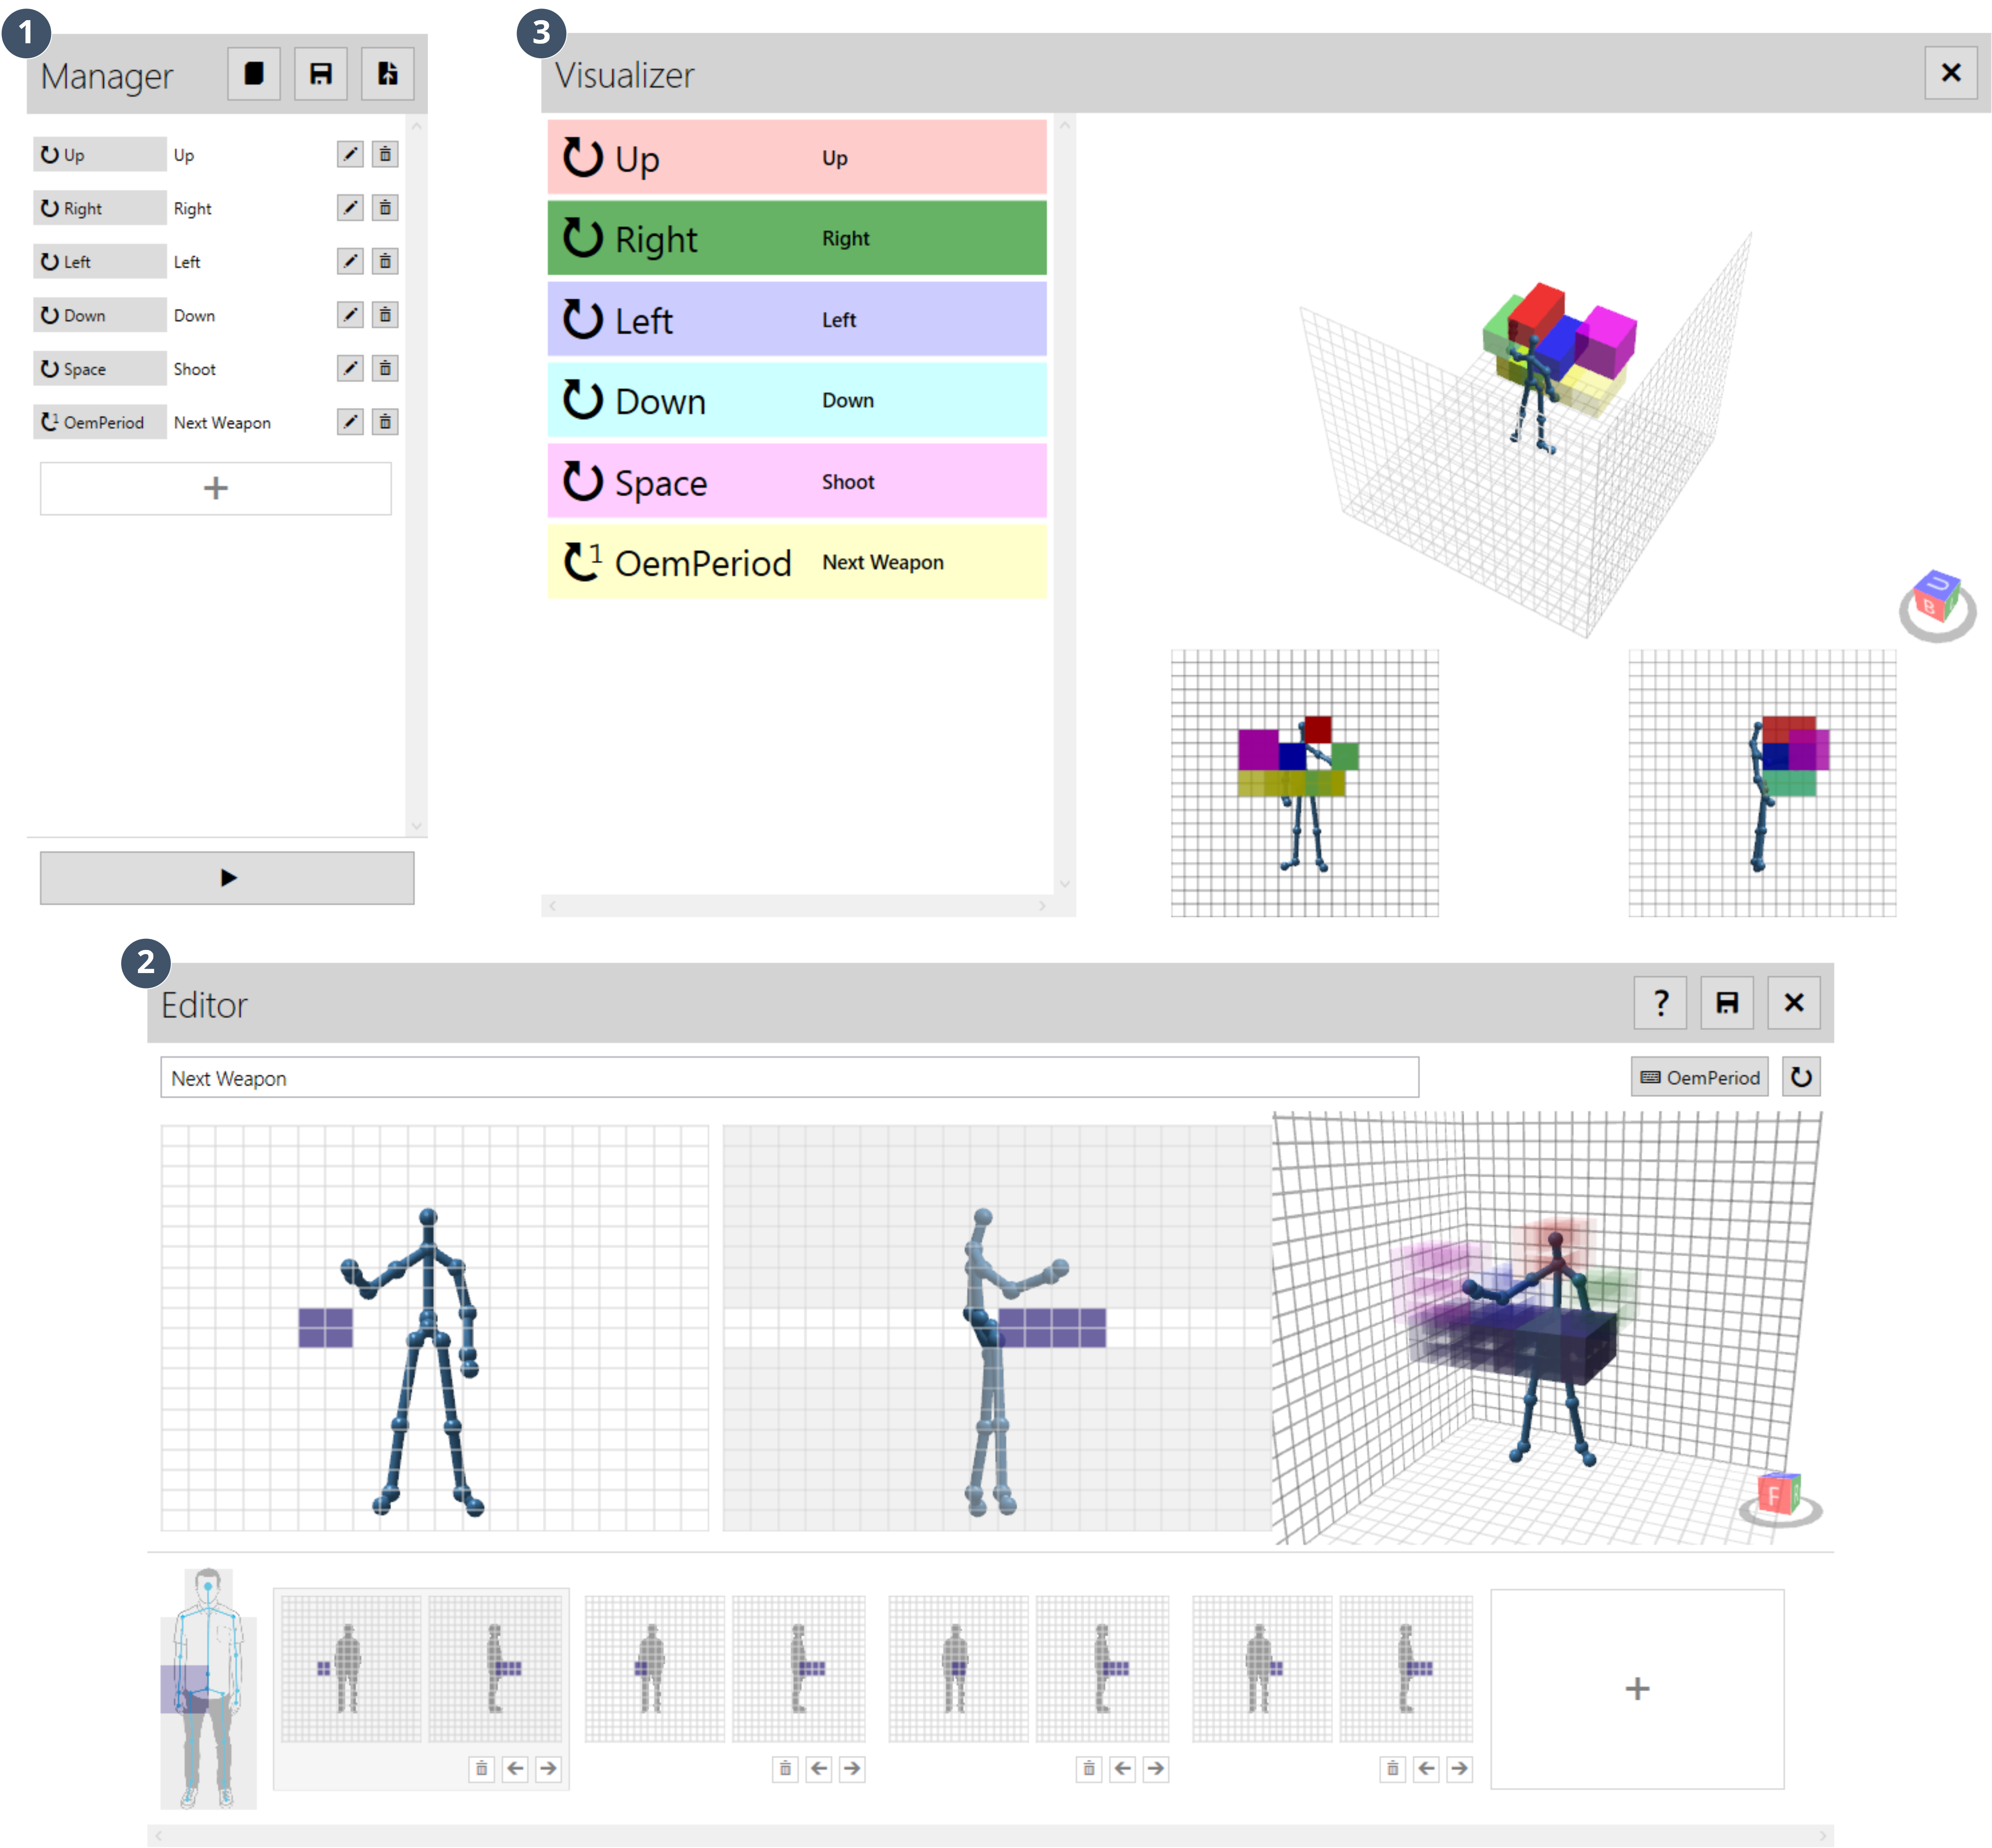
\includegraphics[width=\textwidth]{hotspotizer-modules}
\caption{Hotspotizer consists of three modules: (1) The Manager lists all of the gestures in the current collection and allows creating, saving and loading collections as well as adding, removing and editing individual gestures. (2) The Editor is the main workspace where gestures are authored. (3) The Visualizer provides interactive feedback on available and recognized gestures.}
\label{fig:hotspotizer-modules}
\end{figure}

\subsection{Usage}

To describe how mid-air gestures can be authored and mapped to keyboard events using Hotspotizer, lets consider the case of an end-user, Ali, who would like to adapt a document viewing application for gesture control. (Ali may require this functionality in contexts where touching a device to navigate a document is undesirable; e.g. when performing surgery on a patient or repairing an oily mechanism.) Figure~\ref{fig:workflow} depicts his workflow, and the numbers in parentheses throughout this section relate to the numbered panes in the figure.

\begin{figure}[ht]
\centering
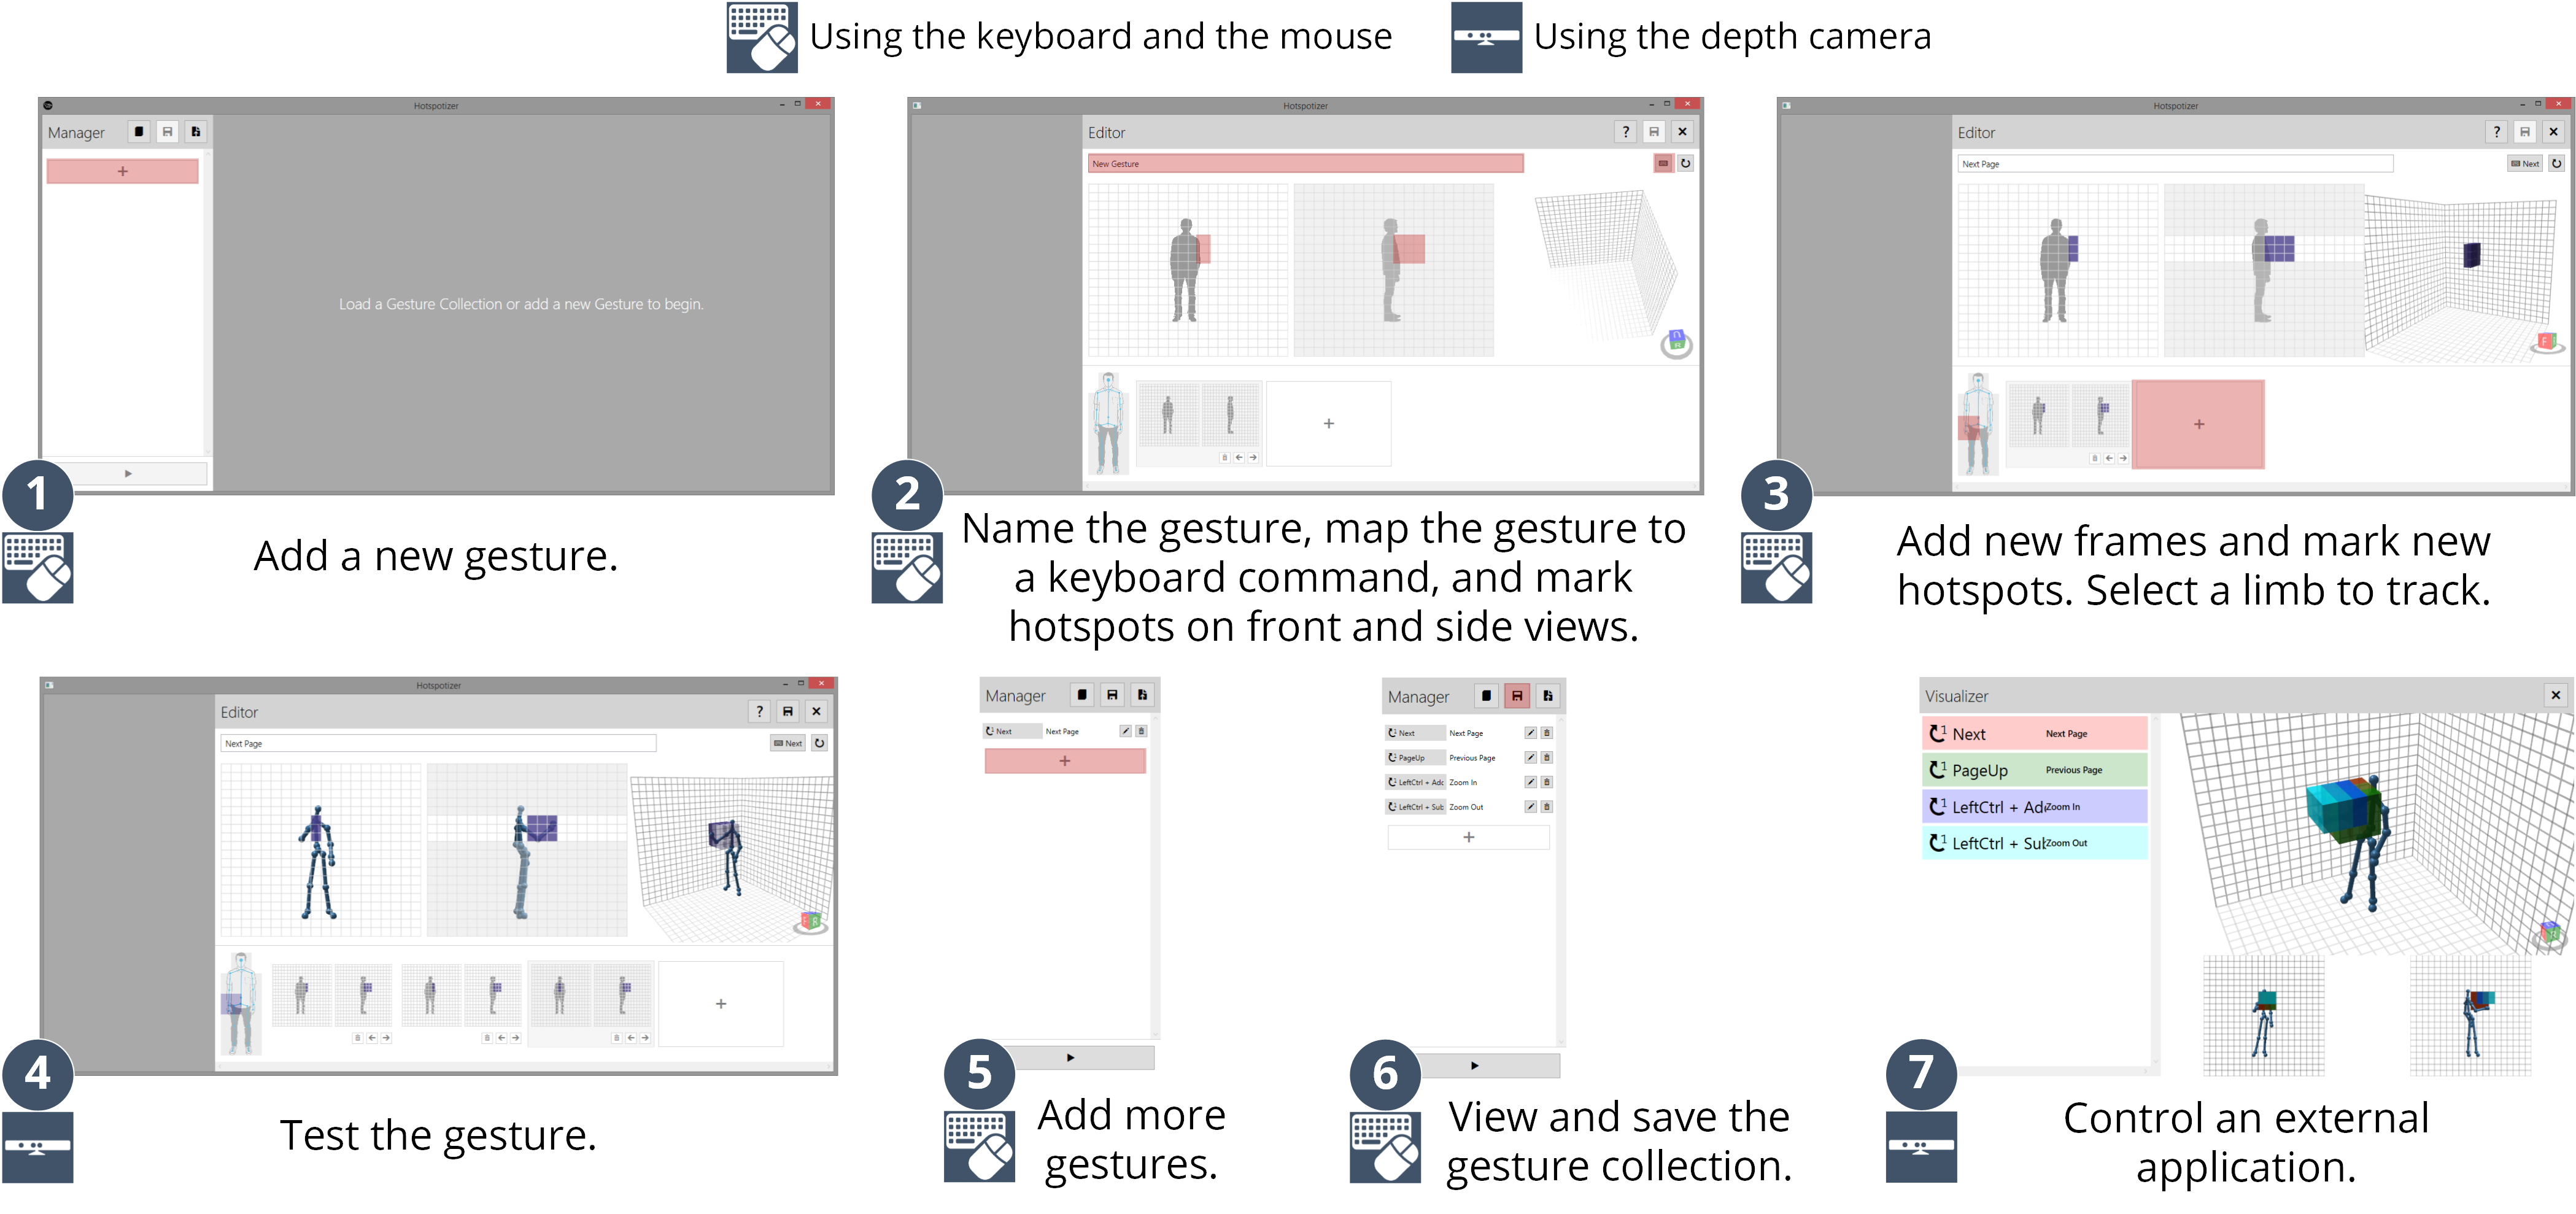
\includegraphics[width=\textwidth]{workflow}
\caption{The workflow of an end-user authoring gestures in Hotspotizer.}
\label{fig:workflow}
\end{figure}

Ali has to be able to cycle up and down between the pages of a document, as well as zoom in and out, using mid-air gestures. These actions may correspond to different keyboard commands depending on the document viewing application; lets assume that, respectively, the \emph{Page Up}, \emph{Page Down} keys and the \emph{Ctrl + Plus} and \emph{Ctrl + Minus} key combinations are used. To cycle between pages, the left hand is swiped in air as if turning the pages of a real, albeit large book. To zoom in and out, the right hand performs beckoning and pushing motions. Figure~\ref{fig:gestures} shows one way of describing these two gestures in terms of hotspots (for brevity, the \emph{page up} and \emph{zoom out} gestures are not shown).

\begin{SCfigure}[\sidecaptionrelwidth][ht]
\centering
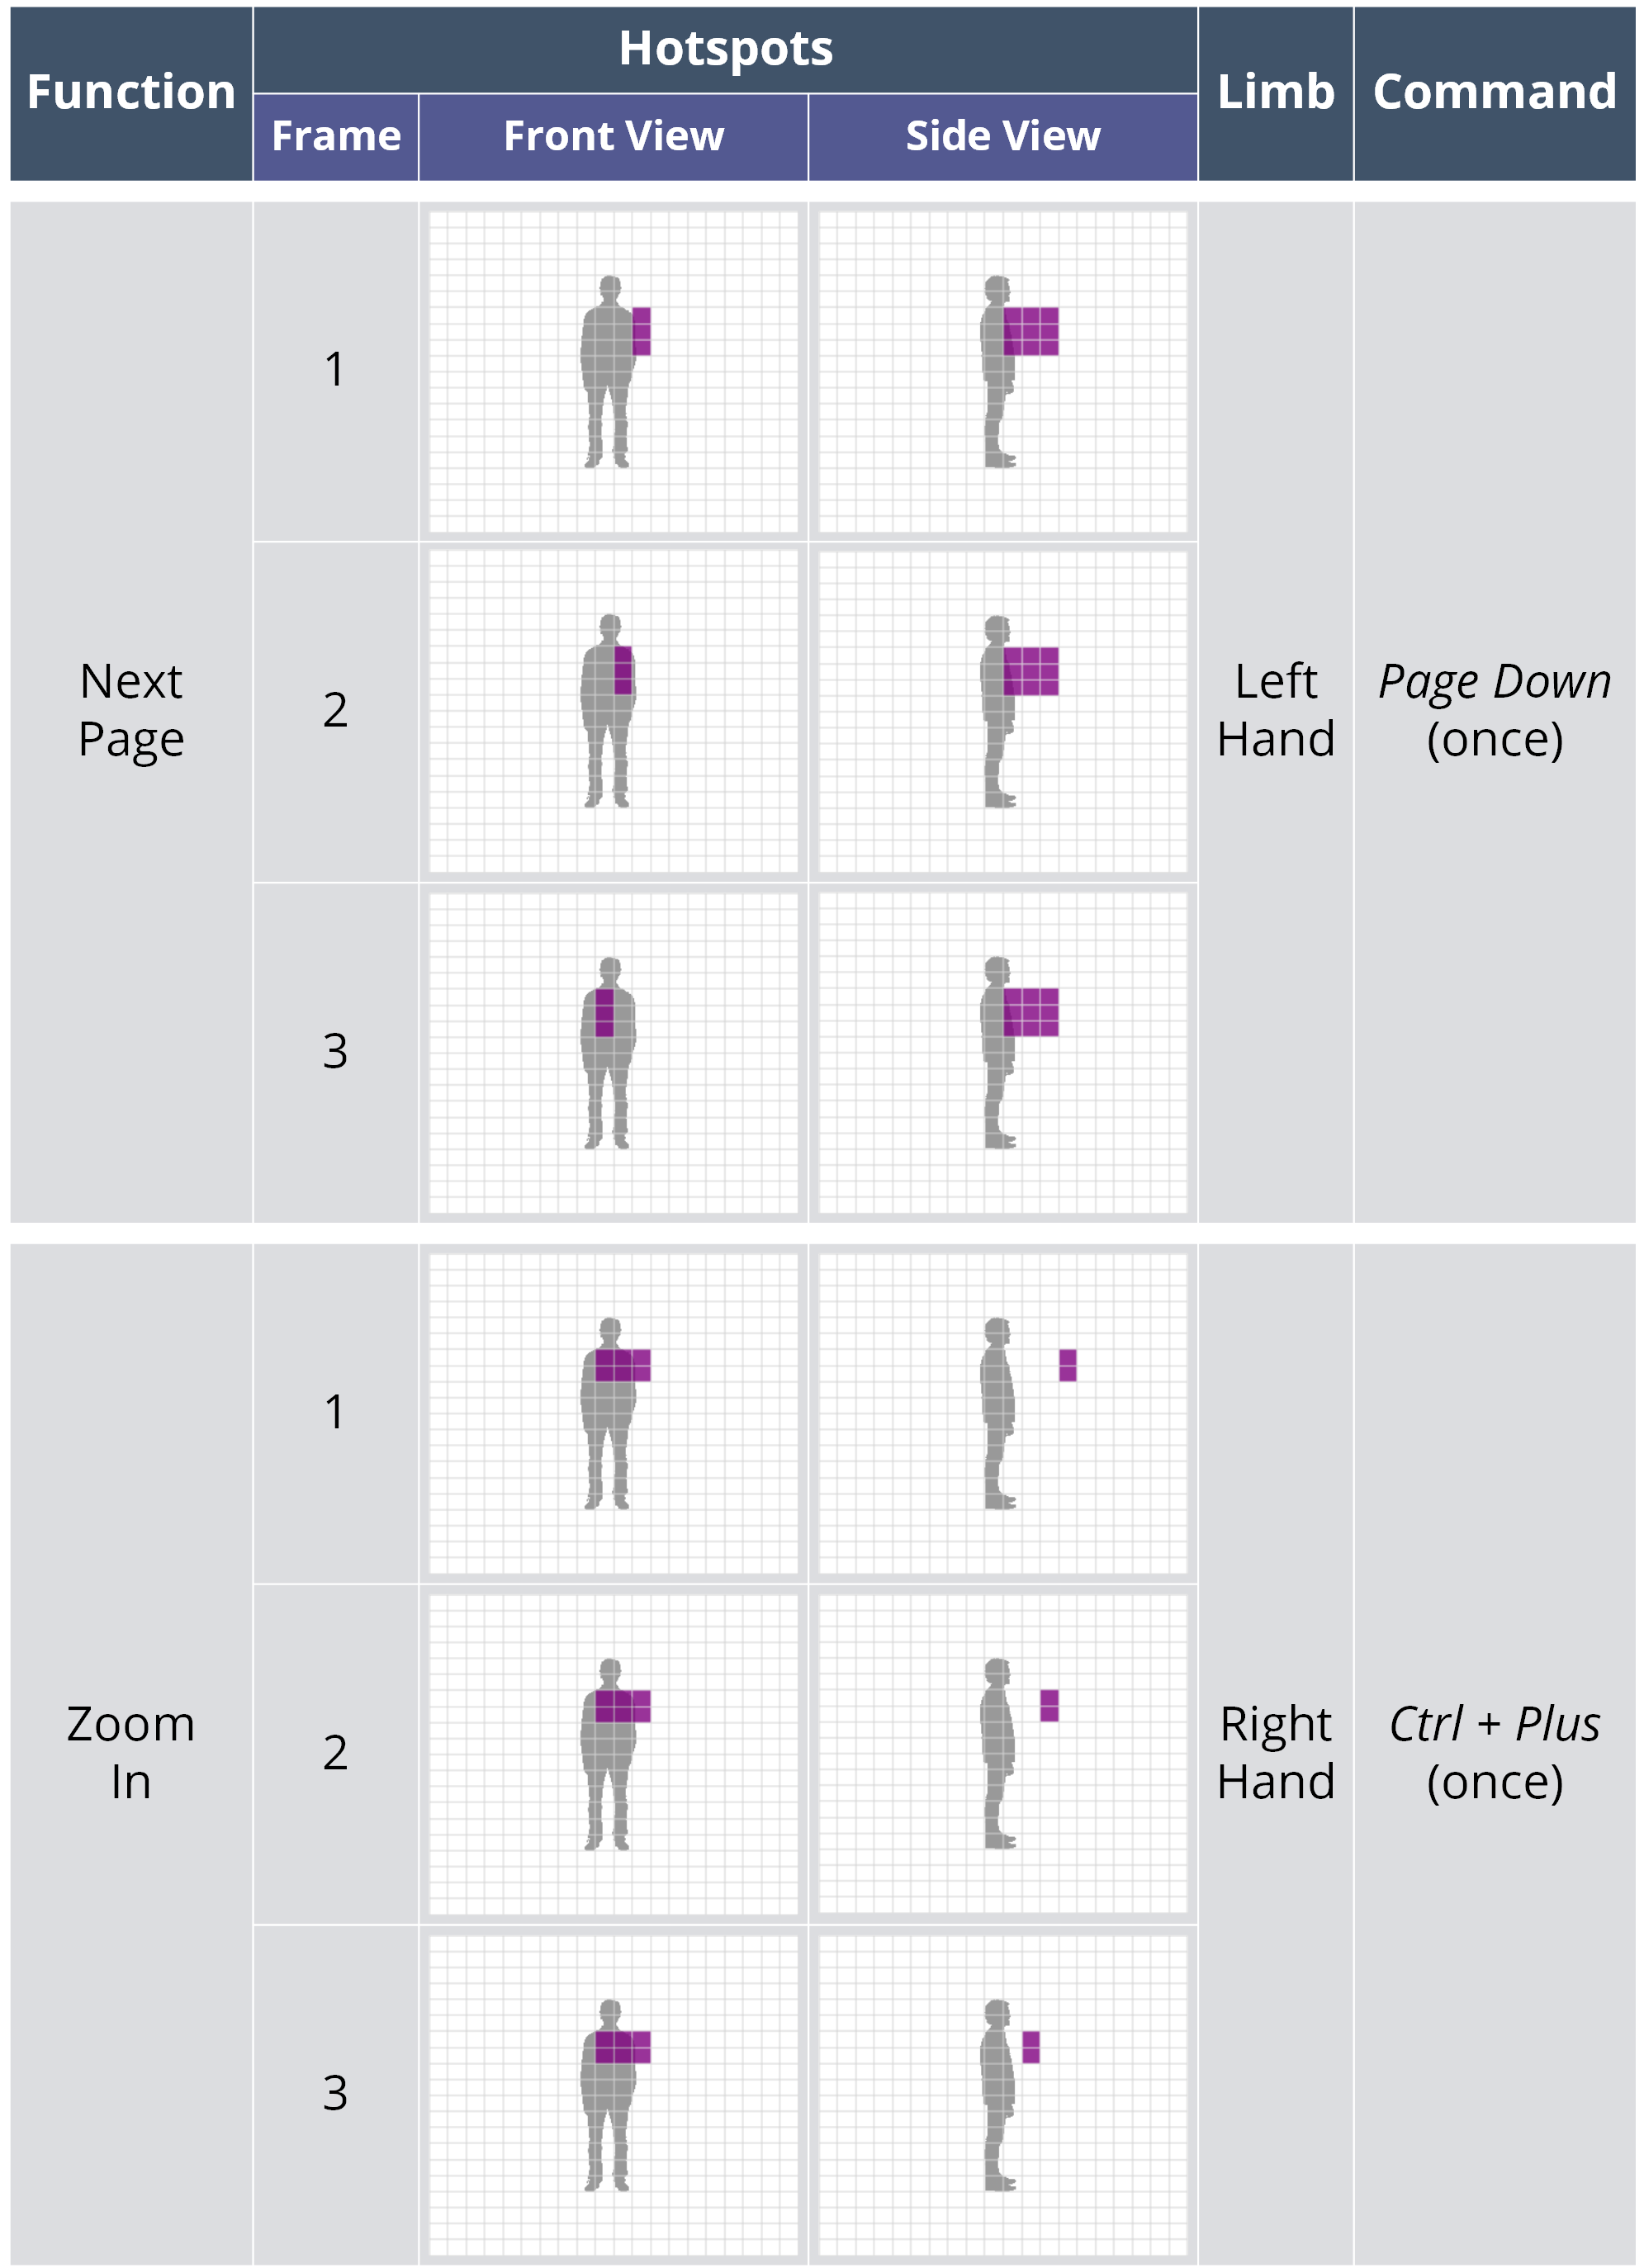
\includegraphics[width=.6\textwidth]{gestures}
\caption{\emph{Next page} and \emph{zoom in} gestures to control a document viewing application and the keyboard functionality that they map to. The diagrams show, respectively, hotspot arrangements for a swipe gesture and a beckoning motion.}
\label{fig:gestures}
\end{SCfigure}

\subsubsection{Creating and Editing Gestures}

Hotspotizer greets Ali with the Manager module containing empty gesture collection upon launch. Ali creates a new gesture in the collection, launching the Editor module \textbf{(1)}. Here, Ali assigns a name for the gesture for easy recall, specifies the Page Down key to be triggered when the gesture is performed, and confirms that the \emph{loop} toggle button is not checked – otherwise performing the gesture and holding the tracked limb over the hotspots in the last frame continues to hold down the keyboard key assigned to the gesture \textbf{(2)}.

Ali moves on to the main workspace where they use the front- and side-views over a representation of the tracked user to mark the positions of the hotspots for the first frame. Initially, all of the cells in the side view are disabled and grayed out. Marking cells on the front view enables the corresponding rows on the side view, whereupon Ali can mark the vertical and depth-wise position of their hotspots. Once hotspots are specified in all three dimensions by using these two grids, they appear on the 3D viewport on the right.

Once Ali completes marking the first frame’s hotspots, they can proceed to add another frame using the button next to the timeline of keyframes, and then another \textbf{(3)}. Finally, after marking the second and third frames’ hotspots, Ali selects the left hand as the limb that will be used in performing this gesture.

After saving the first gesture into the collection, Ali is taken back to the Manager module where they can add the remaining gestures and see the existing gestures to review, edit or delete them \textbf{(5)}. Once they are satisfied with the gesture collection they created, Ali can save the collection into a file for later use \textbf{(6)}.

\subsubsection{Testing Designs and Controlling External Applications}

At any time when using the Editor module, if they have a Kinect sensor connected to the computer, Ali may step in front of the sensor and see a rendering of the skeletal model of their body on the front, side and 3D viewports \textbf{(4)}. This feature can be used to rapidly test and tune hotspot locations at design time.

Testing over the whole gesture collection is available through the Visualizer module \textbf{(7)}. This module depicts a list of the gestures in the current collection and all of their hotspots on 3D, front and side viewports. Each gesture is shown in a different color. On the 3D viewport, transparency implies the order of hotspots. Hotspots glow when the tracked limb enters them in the correct order.

The Visualizer module also embeds the keyboard simulator. Launching the visualizer attaches a virtual keyboard to the system, which relays associated key events upon the successful performance of gestures. The visualization and the emulator continue to work when Hotspotizer is not in focus or is minimized.

\subsection{Implementation Details}

Hotspotizer was written in the \emph{C\#} programming language\footnote{\href{http://msdn.microsoft.com/en-us/library/kx37x362.aspx}{msdn.microsoft.com/library/kx37x362}}, using the \emph{Microsoft .NET Framework 4.5}\footnote{\href{http://www.microsoft.com/net}{microsoft.com/net}} and the \emph{Windows Presentation Foundation (WPF)}\footnote{\href{http://msdn.microsoft.com/en-us/library/ms754130.aspx}{msdn.microsoft.com/library/ms754130}} subsystem therein to create the user interface.

The following open source packages were used:

\begin{itemize}
\item \emph{Windows Input Simulator}\footnote{\href{http://inputsimulator.codeplex.com/}{inputsimulator.codeplex.com}} for keyboard emulation;
\item \emph{Json.NET}\footnote{\href{http://json.codeplex.com/}{json.codeplex.com}} for reading and writing gesture data to files; and,
\item \emph{Helix 3D Toolkit}\footnote{\href{http://helixtoolkit.codeplex.com/}{helixtoolkit.codeplex.com}} for 3D graphics.
\end{itemize}

Hotspotizer runs on Microsoft's \emph{Windows 7} and \emph{Windows 8} operating systems and requires the \emph{Microsoft Kinect Runtime}\footnote{\href{http://www.microsoft.com/en-us/download/details.aspx?id=40277}{microsoft.com/download/details.aspx?id=40277}}, and, if used with an \emph{Xbox Kinect} sensor, the \emph{Kinect SDK}\footnote{\href{http://www.microsoft.com/en-us/download/details.aspx?id=40278}{microsoft.com/download/details.aspx?id=40278}} to be installed on the user's computer.

We took care to make the process of installing and running Hotspotizer as straightforward as possible, in order to accommodate diverse user populations. We packaged it as a Windows application that can, as convention dictates, be installed from a single executable installer file, launched from the \emph{Start Menu}, and uninstalled from the operating system's \emph{Control Panel}. Upon launch, Hotspotizer checks for its external requirements, the Kinect Runtime and SDK. If the requirements are unavailable, it prompts the user to install them, providing links to the web pages where they can be downloaded (Figure~\ref{fig:warning-message}).

\begin{SCfigure}[3][ht]
\centering
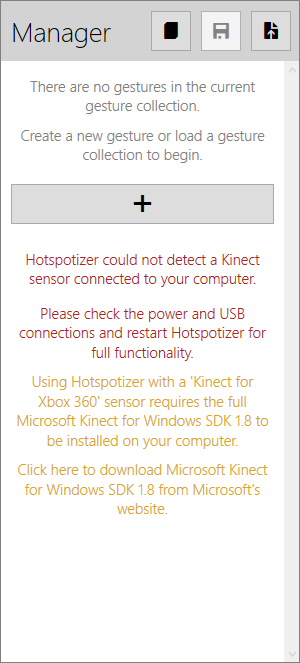
\includegraphics[width=.3\textwidth]{warning-message}
\caption{If the Kinect sensor is not functioning properly or if pre-requisite software is not installed on the computer, Hotspotizer prompts the user with a warning message.}
\label{fig:warning-message}
\end{SCfigure}

\subsection{Discussion}

The space discretization paradigm and its current implementation in Hotspotizer feature strengths and limitations that manifest as side effects of design choices.

One strength of the implementation is that gesture recognition is not influenced by the user's position and orientation within the sensor's field of view, provided that the depth image is not distorted and the sensor can build an accurate skeletal model of the user. Since the discretized workspace is affixed to the user's hip, hotspot locations are defined relative to the user's own body and the traversal of hotspots is detected properly as long as the skeletal model is built correctly. As a limitation of the depth sensor, skeletal modeling fails under certain conditions; e.g. the user turning their back to the sensor or engaging in contortions, the presence of objects that resemble a human form in the sensor's field of view, etc. Hotspotizer automatically hides the skeletal representation and halts gesture recognition when failures occur, and resumes operation when the sensor provides a skeletal model.

Certain limitations result from the design choice to prioritize leveraging a common infrastructure for end-users by mapping gestures to keyboard events. This obscures what \textcite{Hartmann:2007} call "association semantics" --- i.e. the relationship between commands relayed to applications from Hotspotizer and the resulting application behaviors --- and limits the expressive power of the gesture authoring paradigm.

A further limitation is that Hotspotizer currently does not support authoring continuous --- or \emph{online} \parencite{Hoste:2014} --- gestures that affect some variable while they are being performed (as opposed to \emph{offline} gestures that execute commands when the gesture is performed from the beginning to the end). This is not a limitation of the space discretization paradigm; since, theoretically, smaller portions of a gesture could be assigned to affect continuous variables (albeit in a quantized manner). Likewise, gestures that involve pointing at or manipulating dynamic user interface components in third party applications are not supported. This could be overcome by linking the discretized space model around the user with the virtual space of the user interface. However, these features require integration with a fully featured programming environment or language, which is beyond the design goals for this project. Exploring "tighter integration with application logic" \parencite{Hartmann:2007} to empower software developers is a goal for future work.


\chapter{Hotspotizer: Design and Evaluation}
Hotspotizer has been developed through a user-centered design process, in order to fulfill the needs of end-users. This section describes the evolution of Hotspotizer, the evaluation of the final prototype, and insights gained throughout development and deployment.

\section{Formative Studies}
\label{sec:formative-studies}

In the early stages of the design work for a tool to support authoring mid-air gestural interactions, the motivating question was \emph{what} to build. Design efforts were guided largely by qualitative and semi-structured feedback from users and inspiration from related work. Many concepts, in the form of rough sketches and paper prototypes, were produced. Concepts at this early stage included an end-to-end environment for creating gesture-controlled interactive movies that fused gesture authoring and content creation in one application; ready-made widgets that pre-implemented gesture control and plugged into existing development and design environments; and tools to overlay information (such as the distance between two specific joints) onto a visualization of a skeletal model, to complement textual programming.

The rough sketches, paper prototypes and mockups have been presented at a workshop to a group of 10 potential users, aged 22-31 ($\mu$=26), from diverse backgrounds. While recruited from among students and staff of a single university and not representative of a wide demographic, the participants represented the target users of Hotspotizer well. Each had different skills and interests. Among them was an industrial designer, a semi-professional musician, an electronics engineer, a computer scientist, a museum studies student, an interaction designer, a psychologists and a legal consultant. After a presentation on current design tools for mid-air gestural interfaces and our concepts, we collected feedback and made note of new ideas. Although all of the users were self-reportedly familiar with mid-air gestural interaction in the context of gaming, none had any familiarity with existing tools for authoring custom interfaces. Discussions on possible applications for custom gesture control revealed that a modular approach that can interface with a diverse variety of applications is preferable to a full-blown content creation suite. Moreover, even among users engaged in design or programming activities, tools used for these purposes varied greatly. This illustrated the value of a standalone application rather than a tool that generates code in a specific programming language or plugs into a specific environment.

Another round of sketches and prototypes was prepared, some of them higher fidelity, such as a mock screencast showing the use of various modules in a gesture authoring suite. The idea of creating virtual buttons or hotspots in the space around the user and using them to define gestures was depicted in the sketches, as well as an interactive mockup developed in Processing\footnote{\href{http://processing.org/}{processing.org}} (see Figure~\ref{fig:sketches-prototypes}). Other ideas included an application that recognized static poses and a graphical language consisting of atomic primitives for composing gestures. These were presented at a second workshop with the same 10 participants. Here, the concept of space discretization was proposed by a participant, an interaction designer. Upon interacting with the mockup of an interface where free-form areas in space can be made into gesture-tracking hotspots, she commented that she often makes use of squared paper when sketching. Instead of defining free-form regions in space, why not divide space into squares and constrain hotspots to these squares? Further discussion with participants revealed that this paradigm is grasped more easily than composing with atomic actions or constraints, or even demonstration. Moreover, using a visualization of the skeletal model and the space around it allows direct manipulation \parencite{Hutchins:1985}; encapsulates the limitations and prospects of the design space; capitalizes on proprioception; and can mediate interaction through a tight feedback loop \parencite{Wilson:2012}.

\begin{figure}[ht]
\centering
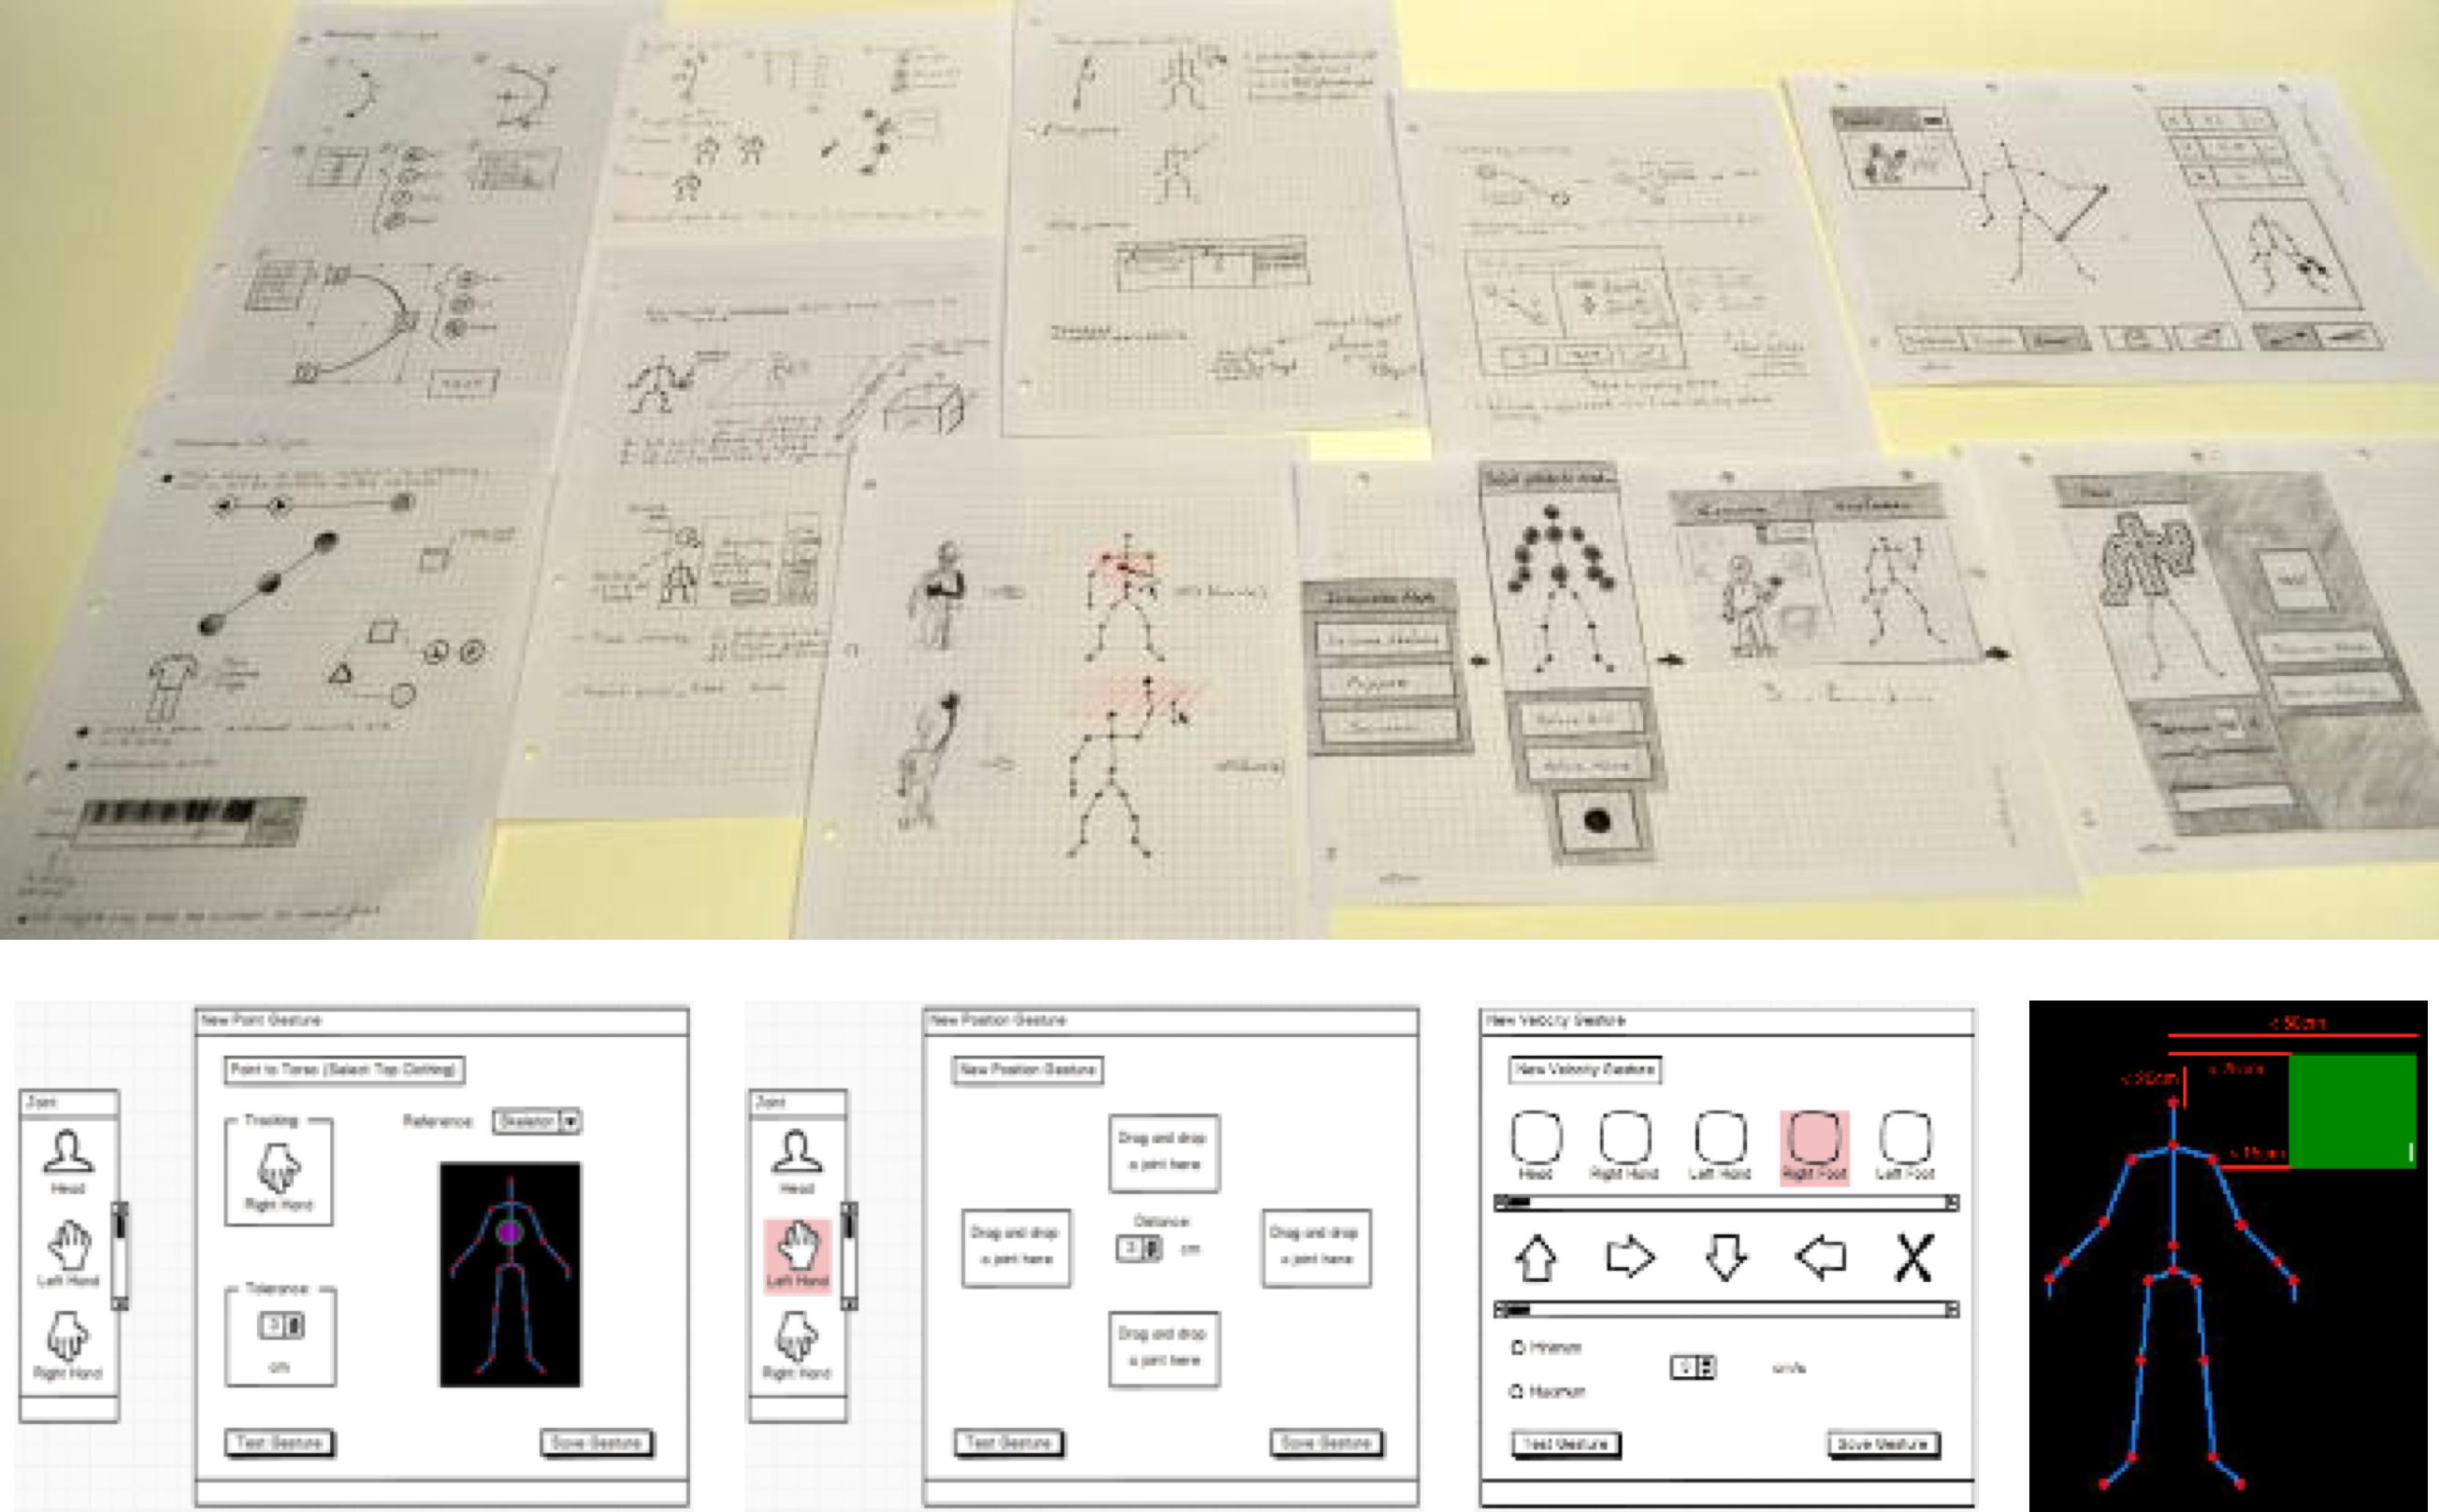
\includegraphics[width=\textwidth]{sketches-prototypes}
\caption{Rough sketches, paper prototypes and mockups were used to gather feedback which directed design and development.}
\label{fig:sketches-prototypes}
\end{figure}

Hotspotizer was developed as an implementation of this \emph{space discretization} paradigm yielded by these workshops. The design guidelines derived from \textcite{Olsen:2007} and \textcite{Shoemaker:2010} were used as filters that transformed the findings from the formative studies into a concrete user interface design. The decision to map gestures to key press events from an emulated keyboard was grounded in \posscite{Olsen:2007} principle for building on an infrastructure that is common across users and situations.

\section{Summative Studies}
\label{sec:summative-studies}

To evaluate Hotspotizer in use, two studies were conducted. The first was a study with 5 users to assess if Hotspotizer conforms to its design rationale. The second was a class workshop with 6 students working in pairs to build interactive prototypes of gestural interfaces. Qualitative results from these summative studies confirm that Hotspotizer conforms to our design rationale (see Figure~\ref{fig:design-guidelines-satisfied} for a summary of the observations that relate to the design guidelines).

\begin{SCfigure}[\sidecaptionrelwidth][ht]
\centering
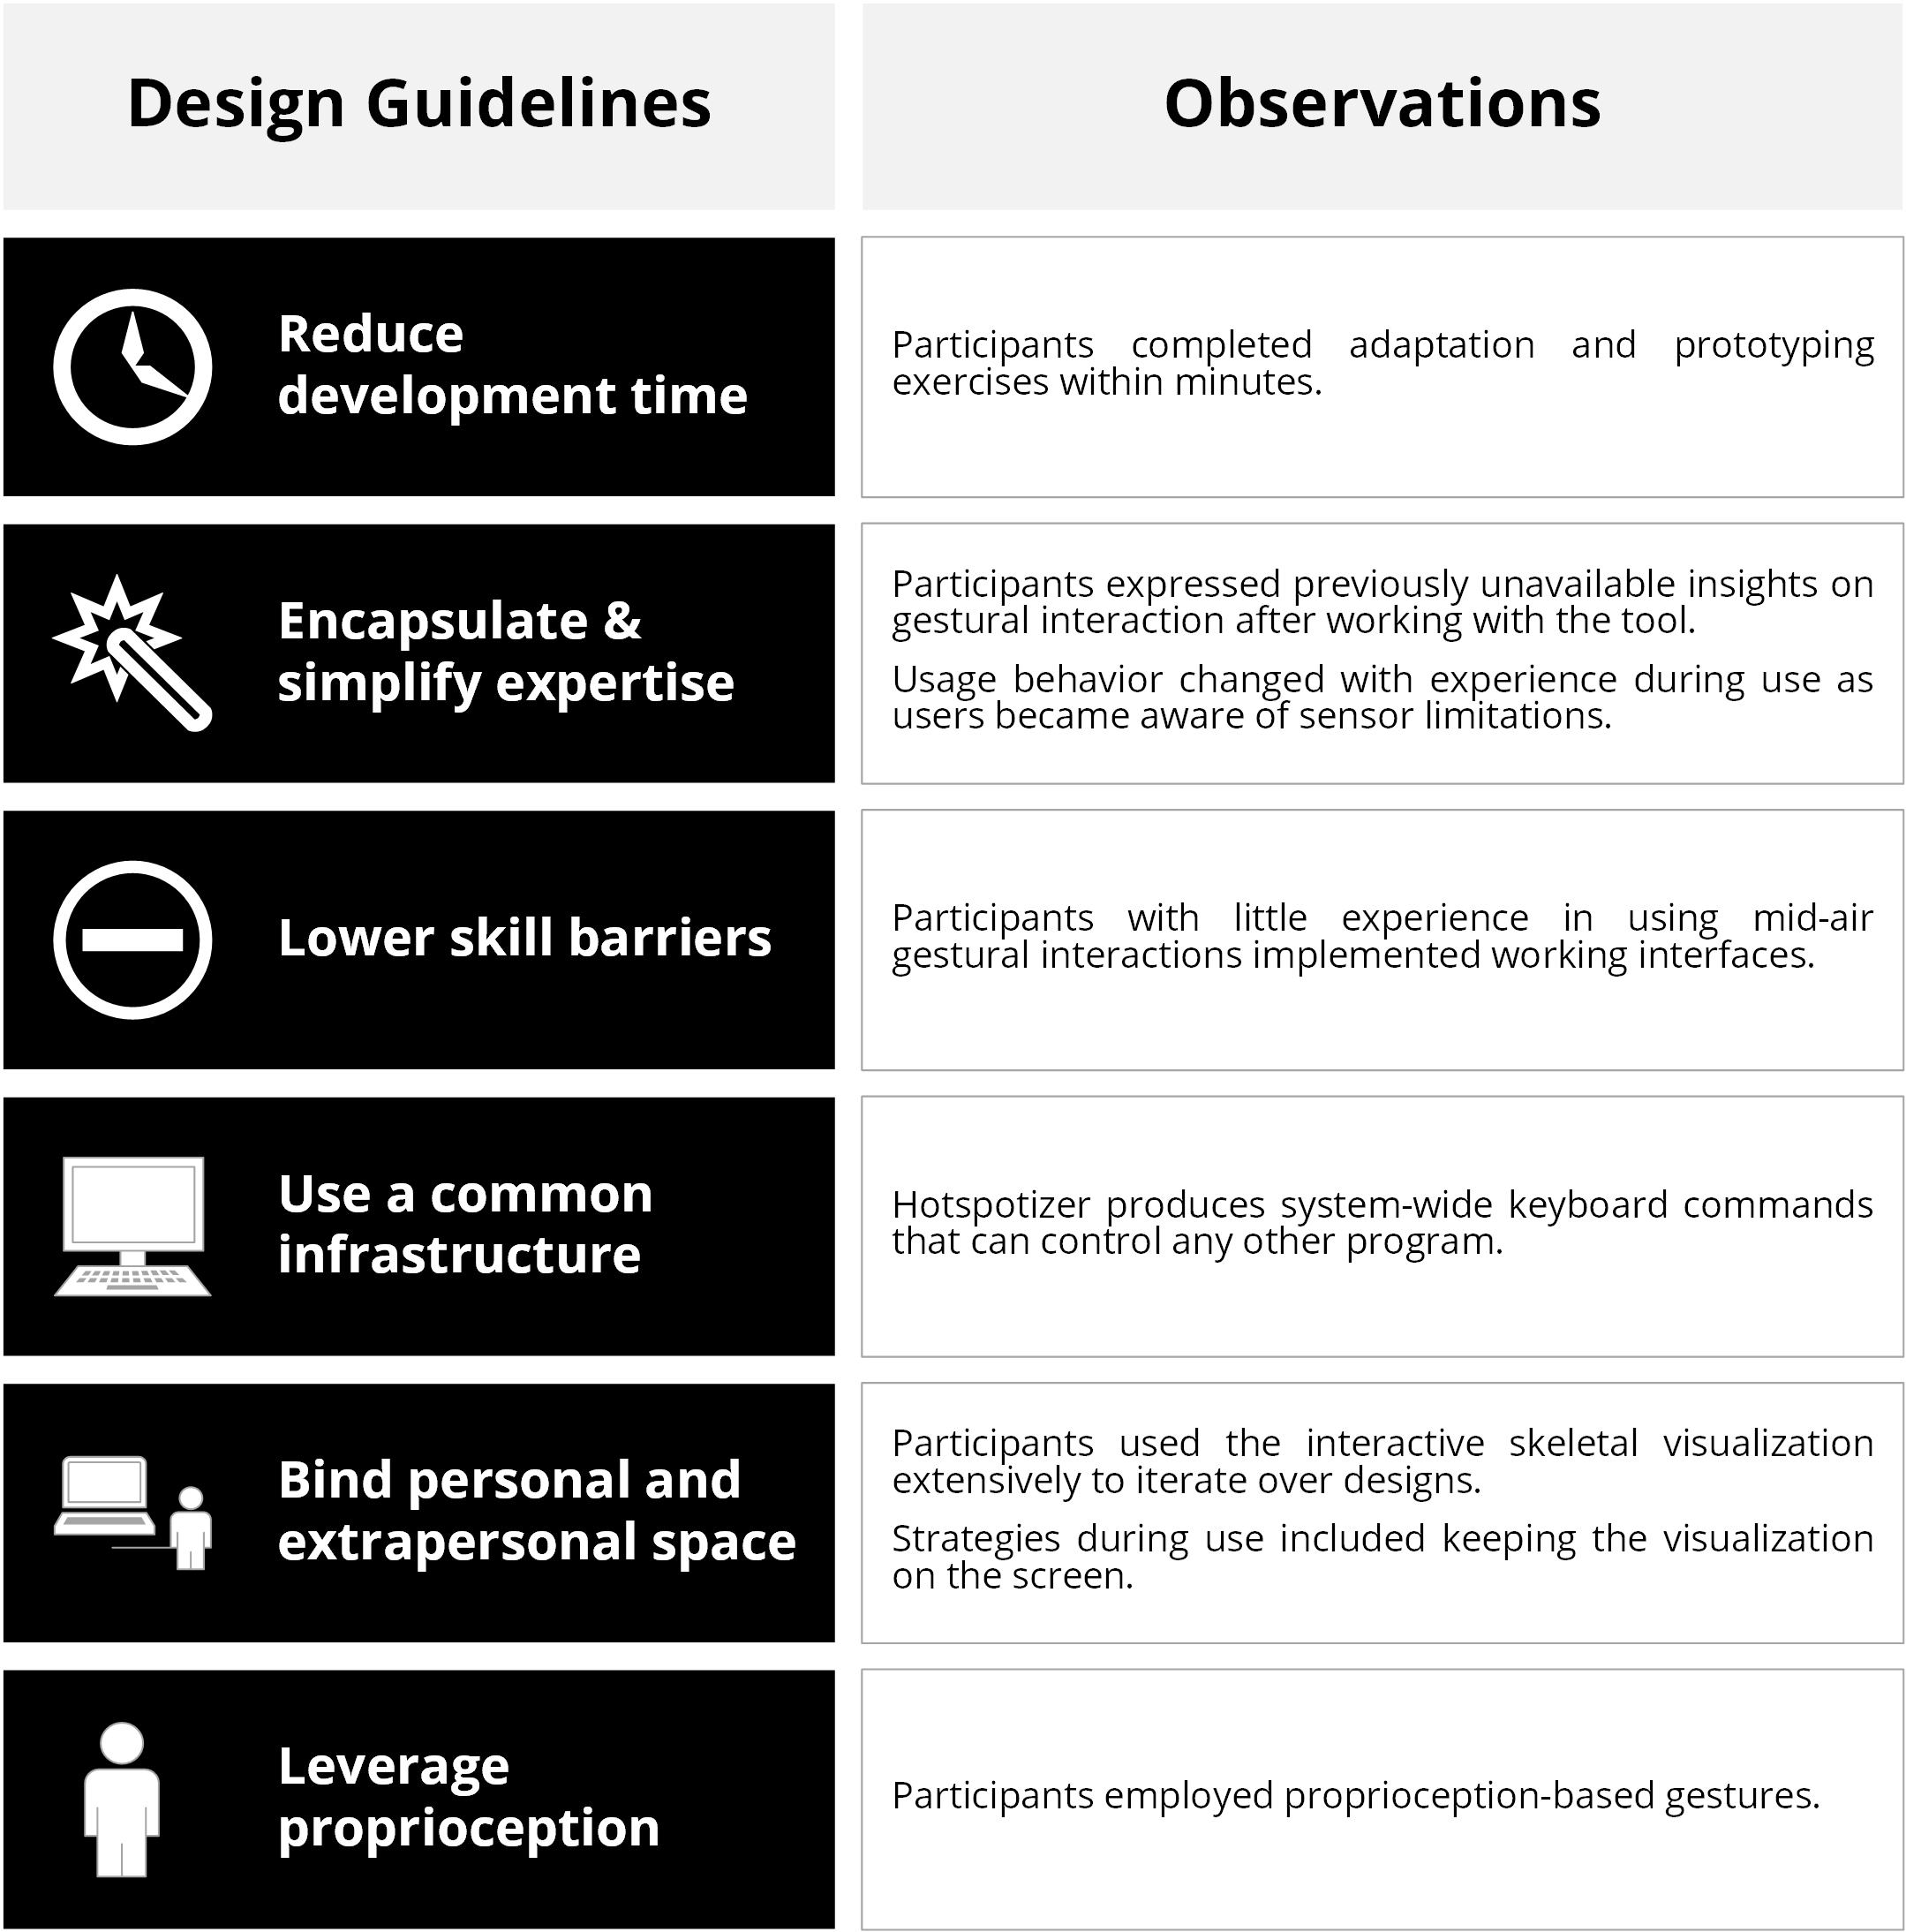
\includegraphics[width=.7\textwidth]{design-guidelines-satisfied}
\caption{Qualitative findings from two studies affirm that Hotspotizer is in keeping with our design rationale.}
\label{fig:design-guidelines-satisfied}
\end{SCfigure}

\subsection{User Study}

For the user study, five graduate students were recruited: an industrial designer, a museum studies student, a computer scientist, a psychologist and an interaction designer. These were not the same people who participated in the previous workshops. Participants were given a pre-study questionnaire where, on average, they self-reported a low level of experience with computer programming ($\mu$=2.1 on a 5-point Likert scale) and a low-medium level of experience with using mid-air gesture-based interfaces ($\mu$=2.4).

Participants were given the task of adapting a non-gestural interface for a computer game to gesture control. They were provided a PC with a Kinect sensor. The game was a side-scrolling platformer --- this style of game was selected since users were expected to be fully familiar with the game mechanics and not be distracted from the process of gesture authoring. The participants were not given specific gestures to implement, but the game required three commands to operate: \emph{left} and \emph{right} for movement, and a \emph{jump} command. Participants were required to play through and complete the first level of the game using gestures. Participants finished the first level using a keyboard and they were gave a demonstration of Hotspotizer before they designed gestures.

All five participants were able to complete the assignment successfully, within 5-14 minutes ($\mu$=7.4min) after being given the demonstration and left alone with the interface. The participants commented that the interface was \emph{“easy to use”} and understandable. Participants iterated rapidly over gesture designs - for each gesture, they went through 2-6 ($\mu$=3) cycles of hotspotizing cells on the Editor and moving into the sensor’s range to test designs. Static hand positions were preferred for the \emph{left} and \emph{right} commands, while the \emph{jump} command inspired diverse gestures including kicking and nodding. A common error across participants was that they marked areas outside the reach of the arms and the legs.

Semi-structured post-study interviews revealed that users had gained insights about the workings of skeletal tracking gestural interfaces. Support for full-body postures such as jumping, along with compositions that involve multiple limbs and grab detection were reported to be desirable as additional features. This is in line with my vision for future work (see Section~\ref{sec:future-work}).

\subsection{Class Workshop}

A workshop was conducted with 6 graduate students taking a course titled “Design Thinking for Interactivity.” Participants worked in groups of two, at the same time. They were given a 20-minute presentation on how the Hotspotizer interface works; and tasked with creating interactive prototypes for three different systems (one per group), following a single given use case for each system. The three systems comprised interactive digital signage for a movie theater, a penalty kick game and a video jukebox for public use. Participants were to create the visual design for the system’s screens in PowerPoint\footnote{\href{http://office.microsoft.com/en-us/powerpoint/}{office.microsoft.com/en-us/powerpoint}}, and assign gestures to shortcut keys in PowerPoint to add interactivity. Each group was provided a Kinect sensor, a PC with Hotspotizer and PowerPoint installed, and a cheat sheet that exposed keyboard commands available in PowerPoint. A diverse set of interactions is possible in this manner, including moving between screens, starting and stopping video, adjusting the volume of the system, displaying versatile animations and automatically triggering timed behavior.

All three groups were able to complete the implementation of an interactive prototype, from scratch, within the 60 minutes allocated for the activity. On average, about one third of this time was spent ideating and sketching designs, one third on composing visuals in PowerPoint and one third on authoring gestures with Hotspotizer. The penalty kick game employed four gestures: kicking a ball towards the left, the right and the center; and making a large circle with the hand to restart. The digital signage prototype was controlled by six hand gestures that involved pointing, swiping, pushing and pulling. The video jukebox prototype was controlled by five gestures that comprised swipes and touching various parts of the head and the torso.

Participants had self-reported low levels of experience with computer programming and using mid-air gestural interfaces ($\mu$=1.8 and $\mu$=2 on a 5-point Likert scale, respectively). They expressed enjoyment from the process of creating interactivity and working with new interface technology. \emph{“A few days ago I did not even know that [mid-air gesture control] was possible. Now I just made my own working design,”} commented one participant.

Initially, users did struggle to understand the workings of the skeletal tracking. Two groups attempted to use gestures with minute differences that the Kinect sensor may not distinguish from each other, such as touching the eye with one finger versus touching the nose. Through trial and error, participants revised their gesture designs to match the capabilities of the sensor.

A limitation to the space discretization paradigm was expected to surface: Hotspots configured for one user could be inappropriate for another user due to differences in body size. After the three groups completed their projects, they tried out each other’s implementations to see if this was the case. The only time when gestures from a new user were not recognized was in the case of the football game, where large leg movements were involved. Differences in the length of the legs hindered gesture recognition across users. Tuning the gesture design to involve larger hotspot areas alleviated the problem. When using hand gestures, no issues were apparent.

\begin{SCfigure}[\sidecaptionrelwidth][ht]
\centering
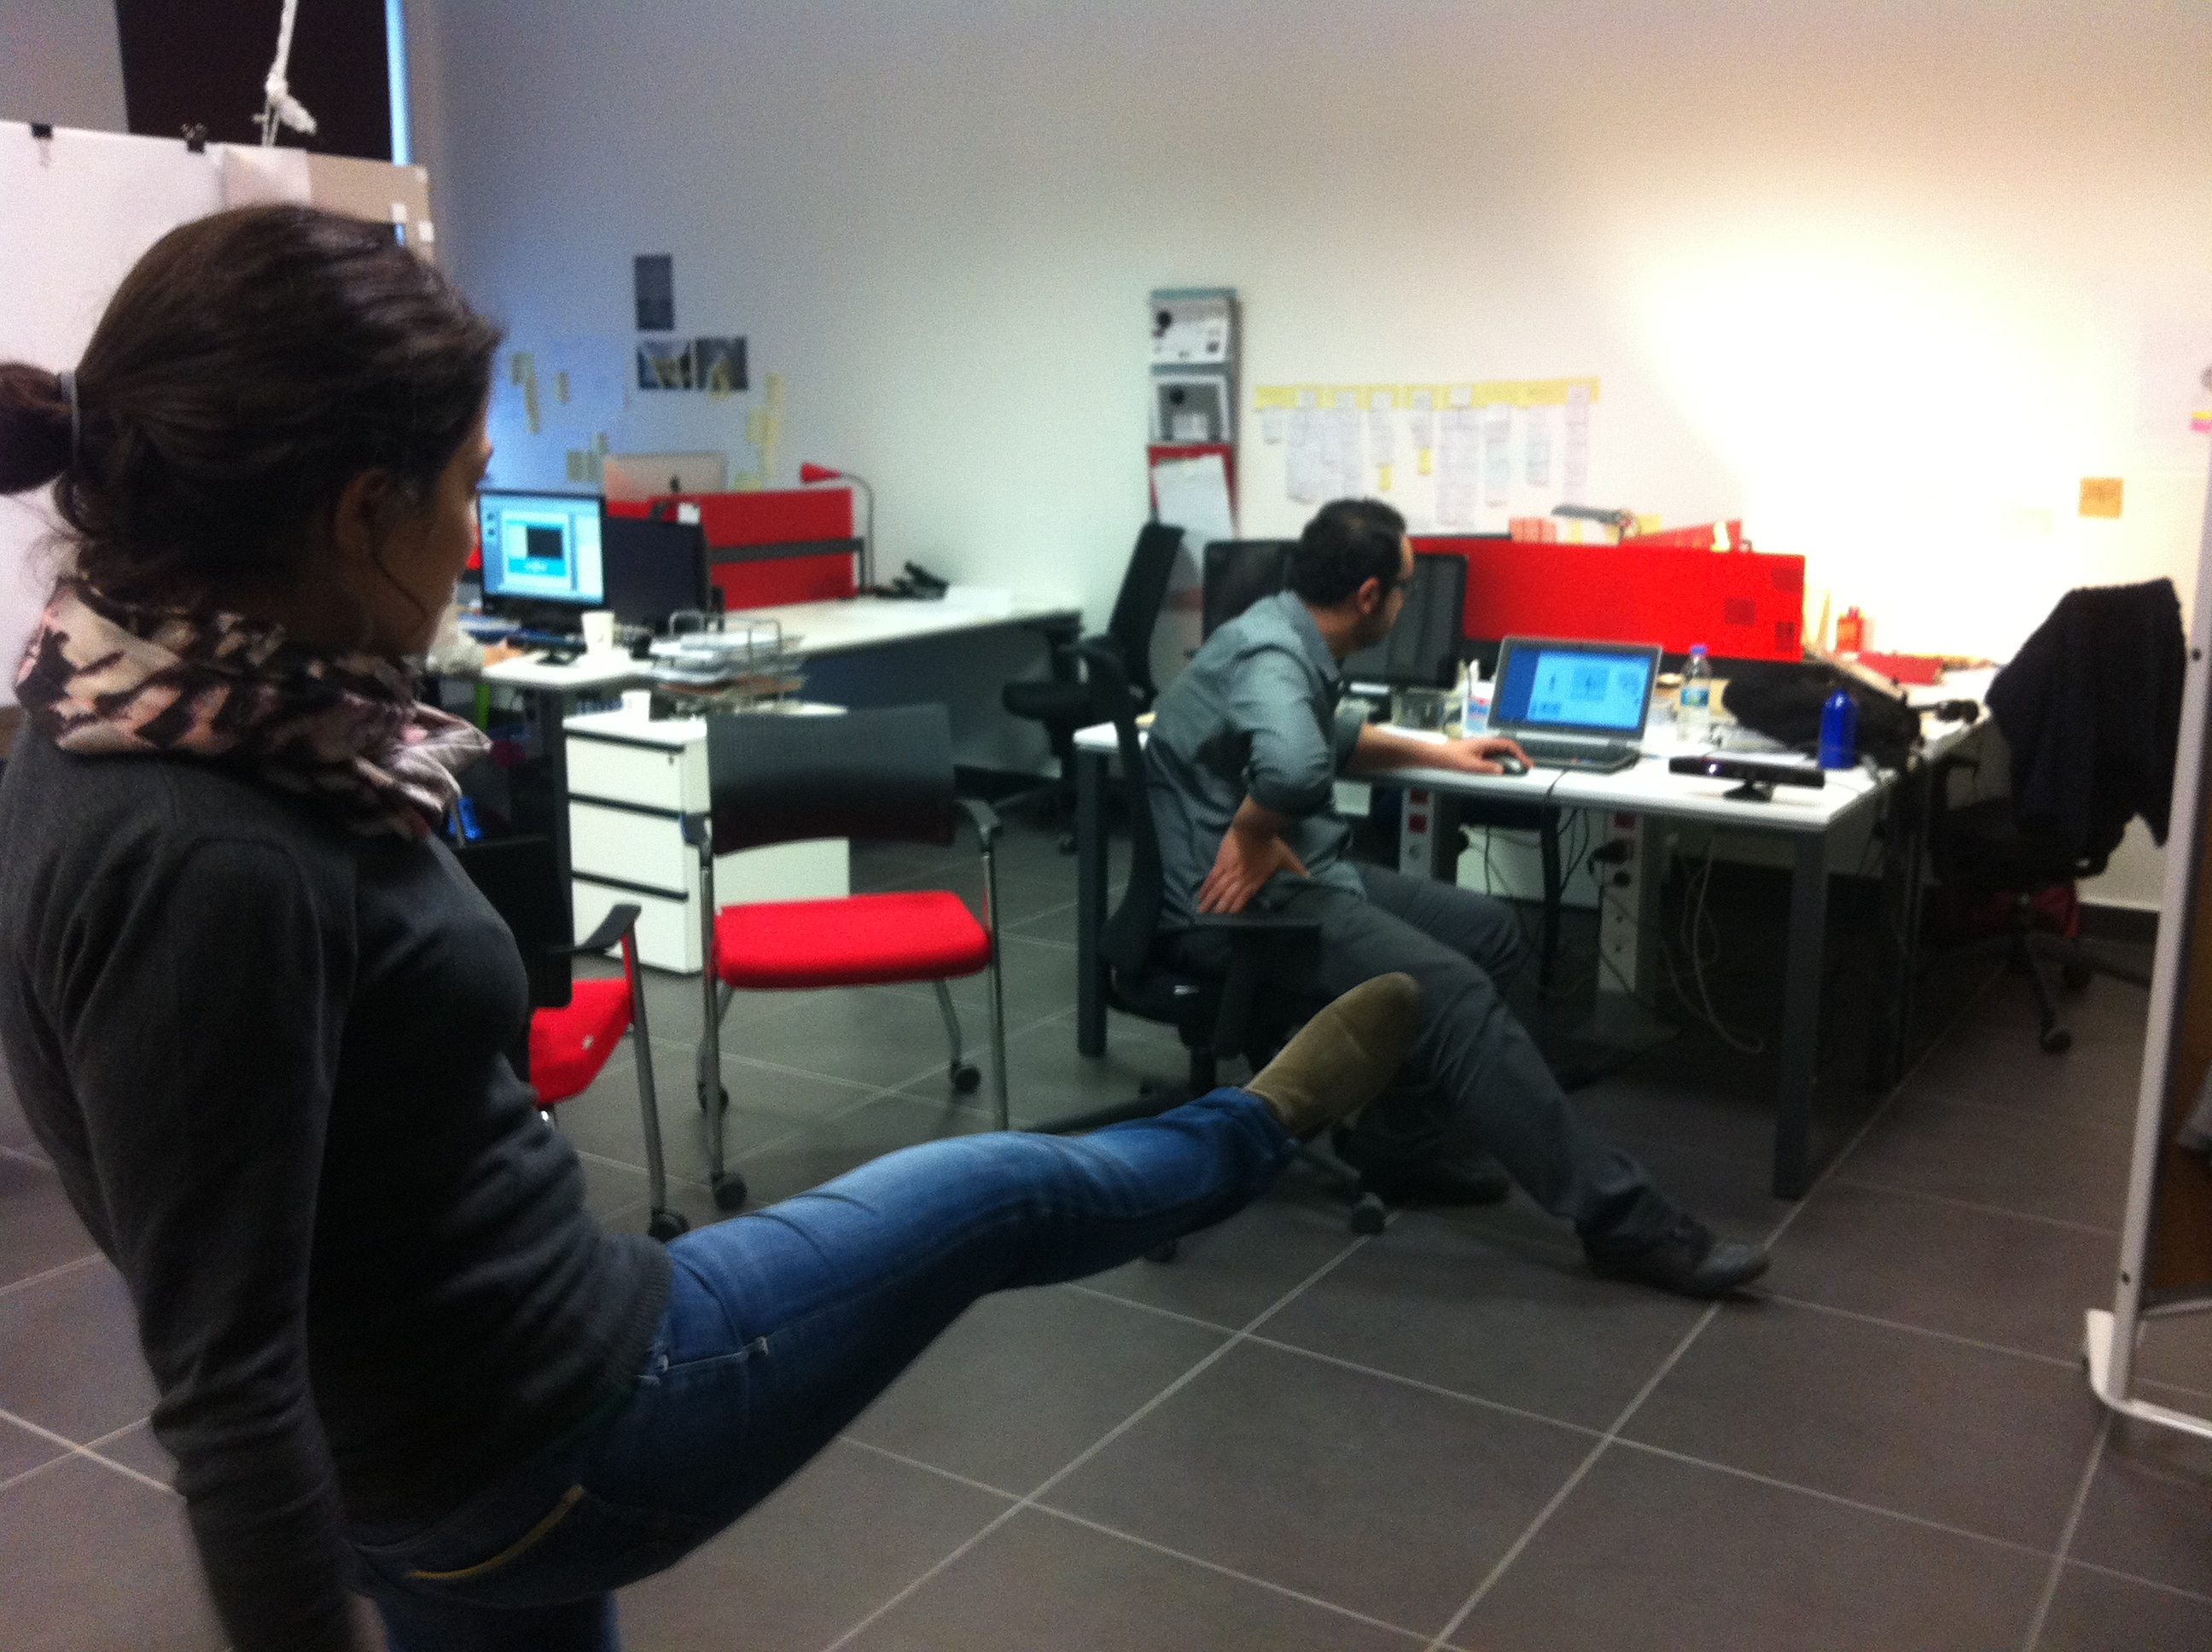
\includegraphics[width=.5\textwidth]{football}
\caption{User strategies included working in pairs. One user performs gestures in front of the sensor while the other marks hotspots that correspond to limb positions.}
\label{fig:football}
\end{SCfigure}

When working in pairs rather than alone, users adopted a different strategy when editing gestures: A single user would mark hotspots using the static on-screen silhouette of a human body as a reference and then test using the interactive representation. Working in pairs, one of the users preferred to stand in front of the sensor and perform gestures, while the other watched the moving representation on the screen and used it as a reference when marking hotspots (Figure~\ref{fig:football}). To allow a single user to enjoy the advantages of using the interactive skeletal model for authoring, future work can implement the ability to infer hotspots from demonstration, along with voice control to interact with the program from a distance (see Section~\ref{sec:future-work}).

Participants were interviewed after the study, where they suggested that while editing, being able to see where hotspots belonging to previously authored gestures reside could be beneficial. This visualization was later added into the Editor module in a later version of Hotspotizer.

\subsection{Generalizable Observations}

During the summative studies, observations that are relevant for the design of mid-air gestural interfaces in general were encountered.

Users who self-reported little experience with mid-air gestural interfaces (a vast majority among participants) tended to be unaware of the limitations regarding the sensor’s field of view. This manifested as an initial tendency to stand too close to the sensor and perform gestures in areas outside the sensor’s field of view. Within minutes, users adjusted to become aware of the boundaries of the interaction area. To promote users' awareness of the depth sensor's field of view, the depth map provided by the sensor could be displayed on screen, as opposed to displaying the user's skeleton alone.

As they tested and used their own gesture-controlled designs, users tended to keep the Hotspotizer interface open and utilize the on-screen representation of the human skeleton. This confirms that the requirements for including a tight feedback loop and a representation for reporting the user’s actions within space are justified. Based on this observation, I can recommend that interfaces based on mid-air gestures include a representation of the tracked skeleton(s).

In general, when designing gestures, users preferred to start with static poses or specify only the end point of a gesture trajectory, utilizing only one frame to implement their designs. In simple cases, such as in controlling the side-scrolling platformer, these designs did suffice. However, as the quantity and complexity of gestures in the interface increases, this approach results in a high number \emph{false positives} in gesture recognition due to intermediate movements intersecting hotspots. Users, due to inexperience, did not anticipate this. Through trial and error, gesture designs were revised and conflicts were resolved, by adding frames and authoring \emph{movement} further constrain designs. Often, gesture designs resulted in \emph{false negatives} due to spatially overconstrained designs that involved small volumes, requiring precise and accurate performance of gestures. Participants, through trial and error, revised their designs by enlarging hotspotized \emph{volumes} to allow for some degree of ambiguity when performing gestures. The general tendency among users was to initially design gestures that were temporally or \emph{sequentially underconstrained} and \emph{spatially overconstrained}. Designs that minimize conflicts by \emph{introducing sequential constraints} (i.e. more frames) while allowing for some flexibility by \emph{relaxing spatial constraints} (i.e. more hotspots) were observed to be more conducive to robust recognition (see Figure~\ref{fig:constraints}).

\begin{SCfigure}[\sidecaptionrelwidth][ht]
\centering
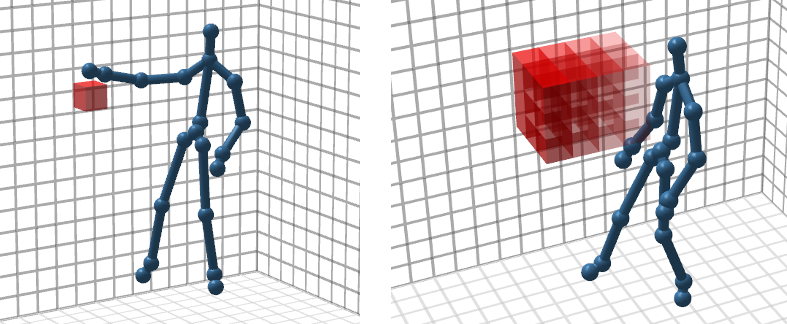
\includegraphics[width=.5\columnwidth]{constraints}
\caption{Initially, users preferred gesture designs that involved small hotspots and unspecified motion. Frames were added to constrain motion, and hotspots were enlarge to allow for variations during gesturing. Here, both panes depict hotspot configurations that may be used for a "punch" gesture. The configuration on the right is more conducive to robust recognition because of its sequentially constrained and spatially relaxed nature, compared to the rather extremely simplistic design on the left.}
\label{fig:constraints}
\end{SCfigure}

\chapter{Conclusion and Future Work}
This thesis described efforts in developing a \emph{software tool for authoring mid-air gestures} to support the activities of end-users. For this purpose, through guidelines derived from the literature and a user-centered design process, a paradigm based on space discretization for visualizing and declaratively manipulating mid-air gesture information was developed. This paradigm was implemented in Hotspotizer, a standalone Windows application that maps mid-air gestures to commands issued from an emulated keyboard.Hotspotizer was evaluated through a user study and class workshop.

Findings from the evaluation sessions verify that Hotspotizer observes its design rationale and supports gesture authoring for end-users. Using Hotspotizer, \emph{gestural interactions were implemented within minutes by users who did not have the skills} to use textual programming tools. Usage strategies and users' choices for gesture designs implied that users understood the \emph{domain expertise} embedded in the interface and leveraged their \emph{sense of personal space and proprioception} in interacting with the system. Hotspotizer was used to control other programs on a PC, making use of a \emph{common infrastructure}.

The space discretization paradigm may have value for authoring gestures enabled using technologies other than skeletal tracking. I encourage other researchers to adopt the paradigm for use in different contexts.

\section{Future Work}
\label{sec:future-work}

The research described in this thesis instigates a number of opportunities for future work.

\subsection{Expanding Hotspotizer}

One strand of future work may deal with expanding the expressive power of Hotspotizer by implementing new features in a user-friendly manner.

While it did not come up in the user studies, I find that the current visualization style may become convoluted as gesture collections grow in size. Exploring alternative ways of visualizing many gestures within one workspace is on our agenda for future versions of the software.

Currently, (as I discussed in Section~\ref{sec:hotspotizer}) Hotspotizer does not directly support "online" (REF) --- i.e. continuous --- gesturing, since it adopts a traditional event-based model for detecting and responding to gestures. As such, support for \emph{manipulative} and \emph{deictic} gestures, which are common across gesture-based user interfaces, is severely limited. As \textcite{Myers:2000} recommend, ideally, the "continuous nature of the input [should] be preserved." This, however, requires "tighter integration with application logic" \parencite{Hartmann:2007} through interfacing with a textual programming language or third-party applications integrating support for continuous input streams. Unfortunately,  the first option oversteps the scope of the Hotspotizer project (See Section~\ref{sec:formative-studies}). The second option can be explored for a limited set of third-party applications.

Among other features are negative hotspots that mark space that should not be engaged when gesturing (i.e. negation \parencite{Hoste:2014}), a movable frame of reference for the workspace to enable gesturing around peripheral body parts, resizable hotspot boundaries, adjustable timeout, compositions that involve multiple limbs, and recognition of hand movements.  As implied by user studies, the capability to infer hotspots from \emph{demonstration}, and \emph{speech recognition} to control the application from a distance are features that may further accelerate user workflows.

Incorporating classifier-coupled gesture recognition \parencite{Hoste:2013} could serve to alleviate recognizer errors \parencite{Myers:2000}, and, when needed, to decouple overlapping gesture definitions.


\printbibliography

\appendix
\chapter{Attributions}

\begin{itemize}
\item Figure~\ref{fig:kinect} by James Pfaff / \href{http://creativecommons.org/licenses/by-sa/3.0/}{CC BY-SA 3.0}
\item Figure~\ref{fig:kinect-gaming} by Sergey Galyonkin / \href{https://creativecommons.org/licenses/by-sa/2.0/}{CC BY-SA 2.0}
\end{itemize}


\end{document}
